\documentclass[english]{article}

% Packages
\usepackage[T1]{fontenc}
\usepackage[bookmarks]{hyperref}
\usepackage{graphicx}
\usepackage{verbatim}
\hypersetup{
colorlinks,
citecolor=black,
filecolor=black,
linkcolor=black,
urlcolor=black
}
% \usepackage[latin1]{inputenc}
\usepackage{amsmath}
\usepackage{amssymb}
\usepackage{amsthm}
\usepackage{enumerate}
% \usepackage{graphicx}
\usepackage{cite}

% Definitions
\def\qqq{\mathbb{Q}}
\def\rrr{\mathbb{R}}
\def\zzz{\mathbb{Z}}
\def\fff{\mathbb{F}}
\def\gftwo{\mathbb{F}_2}
\def\zzzp{\mathbb{Z}_p}
\def\zzzn{\mathbb{Z}_N}
\def\zg{\mathbb{Z}_g}
\def\nnn{\mathbb{N}}
\def\BF{\mathcal{BF}}
\def\xn{(x_n)}
\def\yn{(y_n)}
\def\zn{(z_n)}
\def\an{(a_n)}
\def\Chi{\raisebox{2pt}{$\chi$}}
% \def\qed{$\Box}
% \newcounter{padic}
\newcounter{examples}
\theoremstyle{plain}
\newtheorem{theorem}{Theorem}[section]
\newtheorem{corollary}{Corollary}[section]
\newtheorem{lemma}{Lemma}[section]
\newtheorem{proposition}{Proposition}[section]

\theoremstyle{definition}
\newtheorem{definition}{Definition}[section]
\newtheorem{example}[examples]{Example}

\theoremstyle{remark}
\newtheorem{remark}{Remark}[section]

\begin{document}
\title{On Algebraic Shift Registers}
\author{MIDN 1/C Charles Celerier}

\maketitle

\begin{abstract}
  A stream cipher uses pseudorandom sequences to mimic the security of a
  one-time pad. This paper will investigate how bent functions can be used
  to generate lexicographical bent sequences with large 2-adic valuation.
	Rearrangements of these sequences could be effective for filtering the states
	of feedback with carry shift registers (FCSRs) in stream ciphers. The
	non-linearity of lexicographical bent sequences could provide resistance
  for FCSR-based stream ciphers in register synthesis attacks. In this paper, we
	show that it is possible to compute the 2-adic valuation of a bent
  sequence generated by a Maiorana-McFarland class Boolean function.
\end{abstract}

\section{Introduction}

\par Bytes of data, or short sequences of 1's and 0's, are exchanged between
computer systems all over the planet each day on public channels.
Because gentlemen do read each other's mail, it is necessary to secure the
communication of private data sent over public channels. The solution to this
problem is solved by {\em cryptography}, the designing of systems to secure
data exchanges over public channels.

\par The following example is the same basic communication scenario presented
by Trappe in \cite{trappe-washington_intro-to-crypto}.
Let there be two parties, Alice and Bob, who wish to communicate with one another.
A third party, Eve, is a potential eavesdropper. Alice wants to send a message,
known as the {\em plaintext}, to Bob. To accomplish this without Eve knowing
what the message is before it is received by Bob, Alice must {\em encrypt} her message
by some prearranged method, usually involving an {\em encryption key}, to generate
a related message called {\em ciphertext}. The idea is that the sent ciphertext,
even if it is intercepted by Eve, will be difficult to understand and conceal the
plaintext message. Upon receipt of the ciphertext, Bob will {\em decrypt} the message,
usually involving a {\em decryption key}, similar to the encryption of the message,
and obtain the plaintext message.

\begin{figure}[h!]
	\centering
		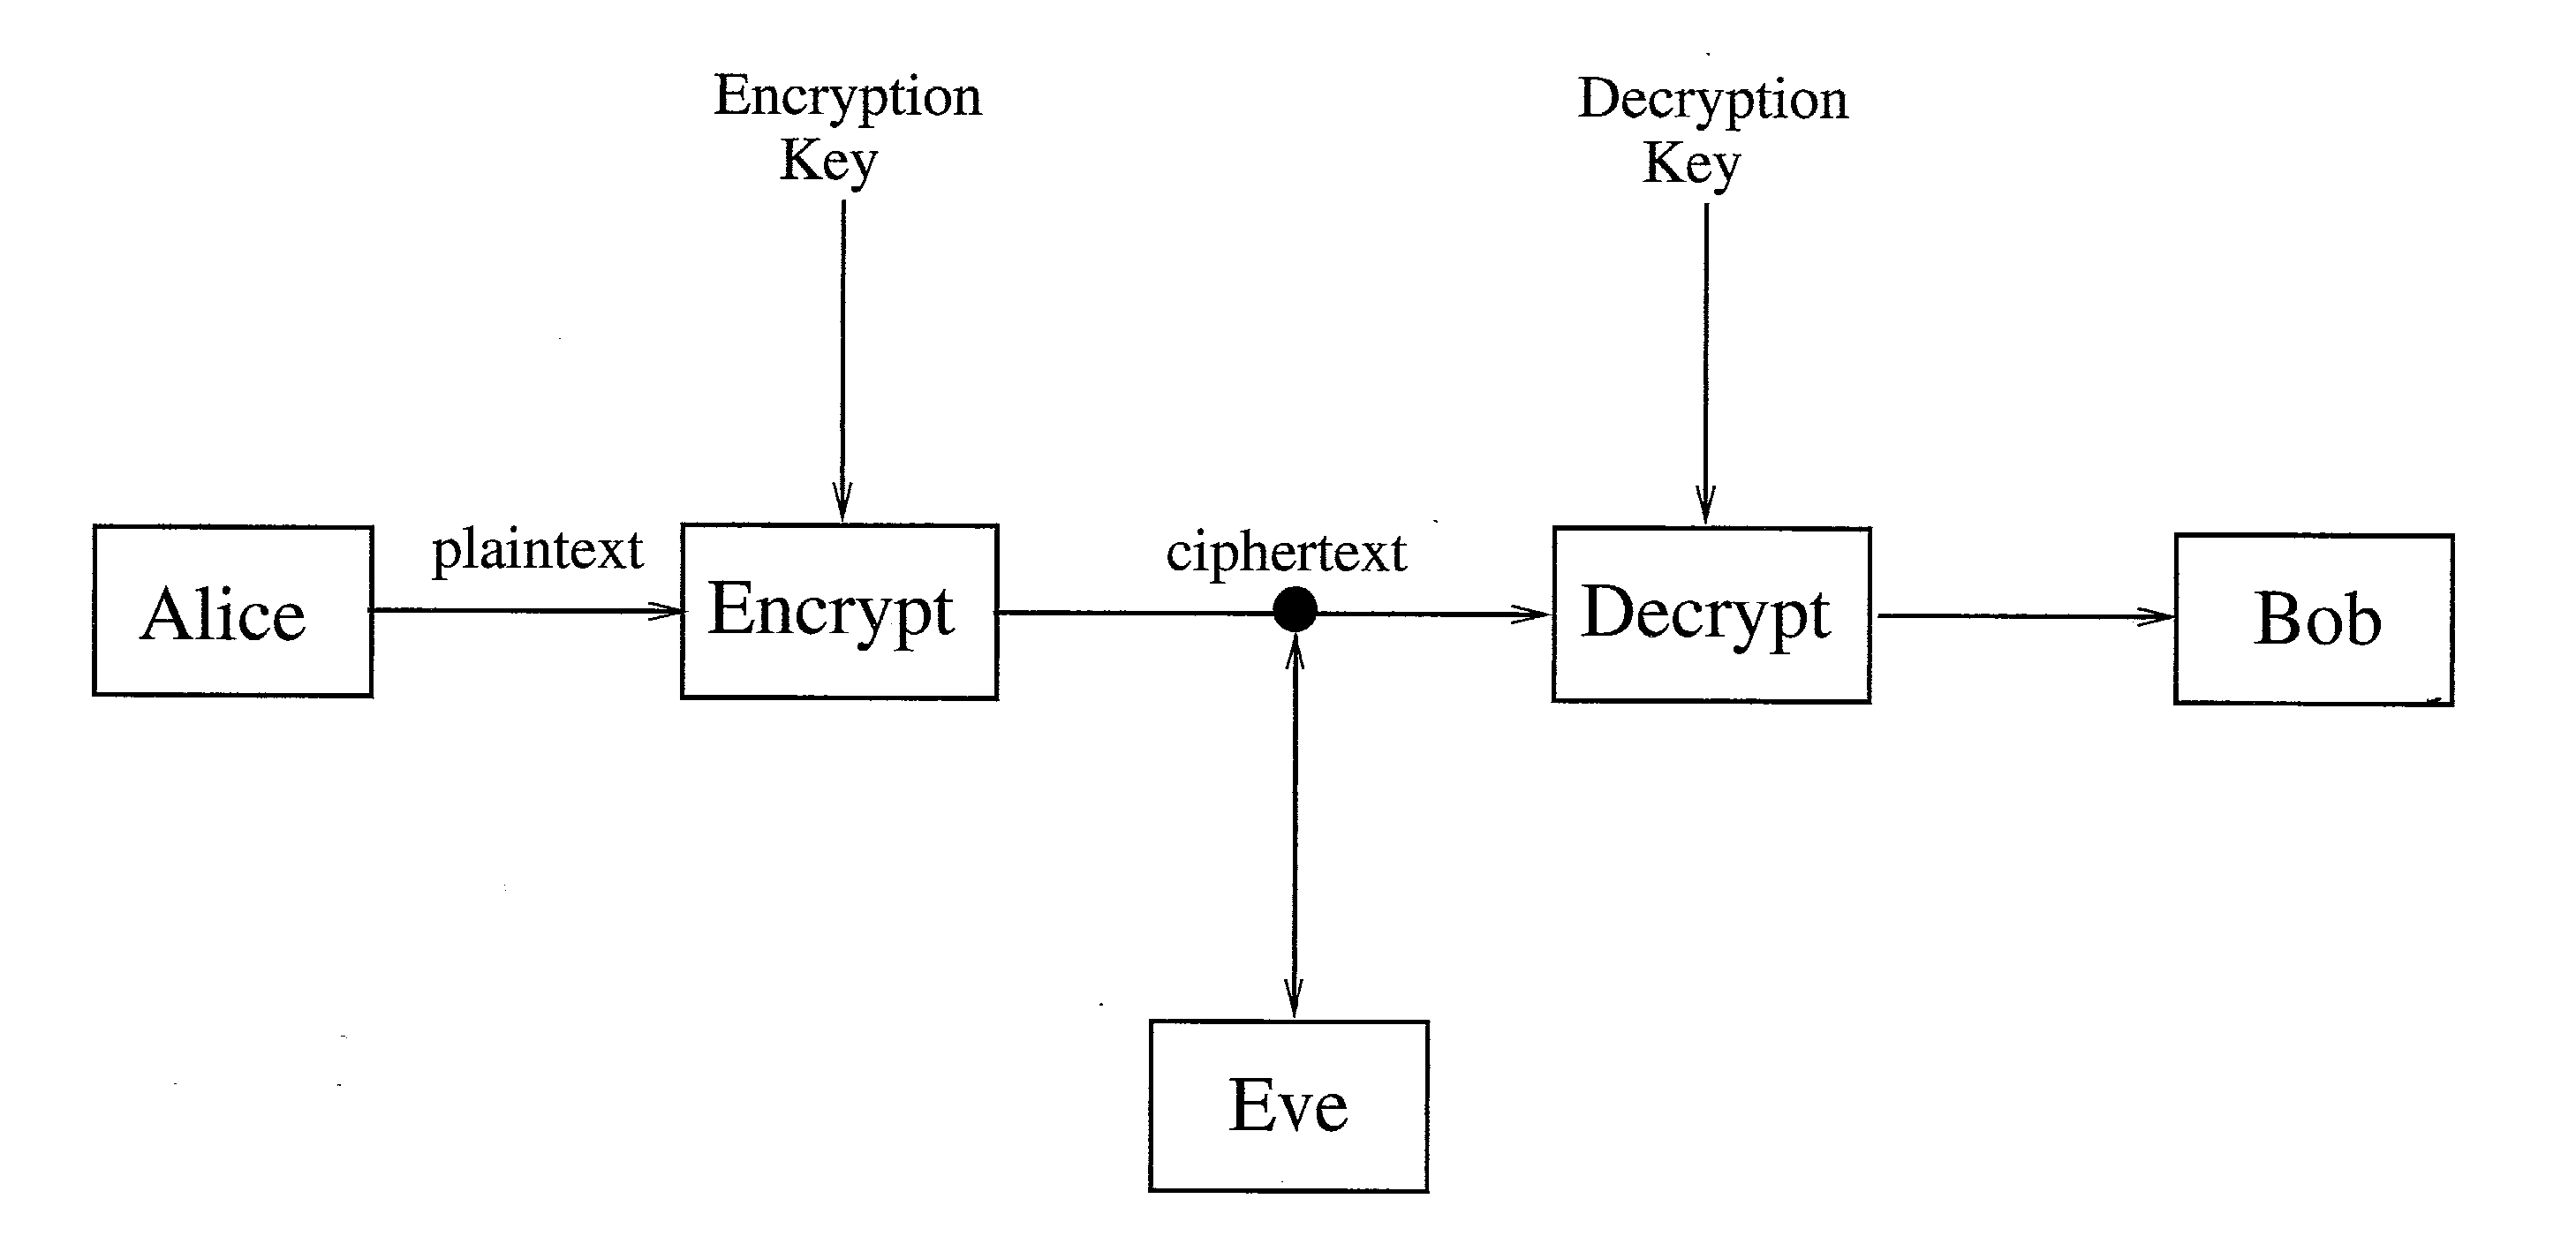
\includegraphics[width=120mm]{figs/basic-scenario.png}
		\caption{The Basic Comunication Scenario for Cryptography \cite{trappe-washington_intro-to-crypto}}
\end{figure}

\par This scenario is the standard example found in many different introductory
cryptography references. Numerous encryption and decryption methods, or {\em cryptosystems},
have been designed to secure the messages sent between Alice and Bob. Unfortunately,
many of these systems have been broken because of the amount of work that goes into
the study of breaking cryptosystems, called {\em cryptanalysis}. A constant battle
exists between the designers and breakers of cryptosystems. In fact, designing
strong cryptosystem typically requires knowledge of cryptography and cryptanalysis.

\par Before diving into the topic of this paper, there is an important assumption that must
be presented. When designing a cryptosystem, every cryptographer assumes {\em Kerckhoffs' principle}:
``In assessing the security of a cryptosystem, one should always assume the enemy knows the method
being used \cite{trappe-washington_intro-to-crypto}.'' The security of a cryptosystem
cannot be based on the concealment of the encryption and decryption algorithms. In practice,
the enemy can obtain the algorithms in many ways, including from the defection or capture
of people. The security must be based on the key and not the algorithm. 

\par Imagine that Alice's message to Bob is a sequence of 1's and 0's, as it would be
in the real world. Consider a cryptosystem which encrypts each bit in the sequence
separately. This would be done by what is called a {\em stream cipher}, which, according to Rueppel,
divides bit sequence into individual bits and enciphers each bit with a time-varying
function whose time-dependency is governed by the internal state of the stream cipher.
The stream cipher can also be thought of in terms of a {\em keystream} which is a
sequence of 1's and 0's the same length of the message that is added to the message
using addition in $\gftwo$ (also known as XOR). If the keystream was perfectly random,
then the cryptosystem would be unbreakable, or {\em perfectly secret}, as
discovered by Claude Shannon in his famous paper ``Communication Theory of Secrecy Systems,''
written in 1945 and published in 1949. This cryptosystem is known as the {\em one-time pad}.
Though it is perfectly secret, it can be difficult to implement because of the inability
to produce perfectly random keystreams. Developing a method to produce perfectly random
sequences is a contradiction in itself. If there is a method to produce the sequence,
then it cannot be perfectly random.

\par Though it is impossible to create perfectly random sequences, it is possible to get close.
This type of sequence is called a {\em pseudorandom sequence}. These sequences have extremely
long periods but are statistically indistinguishable from random sequences. This paper will discuss
the construction of pseudorandom sequences through the use of a particular finite state machine
called the {\em feedback with carry shift register}. It will also investigate the possibility of
incorporating {\em bent functions}, or perfectly non-linear functions, into the construction of
psuedorandom sequences in an attempt to resist synthesizing algorithms. 

\par The paper will follow this basic outline. Important properties of the $p$-adic integers
will be established and examples of different various kinds of $p$-adic integers will be given. 
Then, the finite-state machine will be introduced, followed by the definition of the feedback
with carry shift register. Finally, the boolean functions are defined and described and various
theorems and conjectures will be presented on bent functions.

\section{Boolean Functions}
\par This section will establish the definition of a {\em Boolean function} and introduce
a few different tools used to measure properties of these functions. First, the
finite field with two elements, denoted $\gftwo$, is defined. The definitions and
notations will follow those found in \cite{bk:cs09}.

% Definition of the finited field GF(2)
\par The two element field $(\gftwo,\oplus,\cdot)$ is the set $\{0,1\}$ with defined binary
operations $\oplus$ and $\cdot$, also commonly referred to as the {\em XOR} and
{\em AND} operators, respectively.
\begin{table}[h!]\label{table:GF(2)}
	\centering
	\begin{tabular}{|c|c|}
		\hline
		XOR&AND\\
		\hline
		$0\oplus0:=0$&$0\cdot0:=0$\\
		$0\oplus1:=1$&$0\cdot1:=0$\\
		$1\oplus0:=1$&$1\cdot0:=0$\\
		$1\oplus1:=0$&$1\cdot1:=1$\\
		\hline
	\end{tabular}
	\caption{Binary Operations for $\gftwo$}
\end{table}
\par It should be clear that $(\gftwo,\oplus,\cdot)$ is a commutative ring with an
identity. Additionally, the only non-zero element $1$ is it's own inverse. Therefore
$(\gftwo,\oplus,\cdot)$ is a finite field. The $n$-dimensional vector space over $\gftwo$
will be denoted by $\gftwo^n$, with the usual inner product. Components of these vectors,
the individual 1s and 0s, will be known as {\em bits}. For two vectors $x,y\in\gftwo^n$
where $x=(x_0,\cdots,x_{n-1})$ and $y=(y_0,\cdots,y_{n-1})$, the scalar product in
$\gftwo^n$ will be defined as $x\cdot y\equiv x_0\cdot y_0 \oplus \cdots \oplus x_{n-1}\cdot y_{n-1}$.

\begin{example}
	Let $a,b\in\gftwo^3$ such that $a=(1,0,1)$ and $b=(0,1,1)$ then
	\begin{align*}
		a+b      &=(1\oplus0,0\oplus1,1\oplus1)=(1,1,0) \\
		a\cdot b &=1\cdot0\oplus0\cdot1\oplus1\cdot1=1
	\end{align*}
\end{example}

\par Each vector in $\gftwo^n$ can be uniquely represented by an integer between
$0$ and $2^{n-1}$. The binary representation function $B$ is one-to-one.
\begin{equation}
	B:\gftwo^n\rightarrow\nnn\cup\{0\}\ {\rm such\ that }\ B(u)\equiv \sum_{i=0}^{n-1}u_i\cdot2^i.
\end{equation}

\par This definition of $B$ has created the convention where the {\em low bit} or
{\em least significant bit} appears on the left and the {\em high bit} or {\em most significant bit}
appears on the right. There is another notable function which counts the number of 1s in each
vector.

\begin{definition}
\label{def:Hamming}
	Let $u,v\in\gftwo^n$. Then $wt:\gftwo^n\rightarrow\nnn\cup\{0\}$ is defined by
	\[
	  wt(u):=\sum_{i=0}^{n-1}u_i
	\]
	and $d:\gftwo^n\times\gftwo^n\rightarrow\nnn\cup\{0\}$ is defined by
	\[
	  d(u,v):=w(u+v).
	\]
	Then $wt(u)$ is the {\em Hamming\ weight} of $u$ and $d(u,v)$ is the
	{\em Hamming\ distance} between $u$ and $v$.
\end{definition}

\begin{remark}
	The Hamming weight of a vector $u\in\gftwo^n$ is the number of 1s in the vector, and the
	Hamming distance between two vectors $u,v\in\gftwo^n$ is the number of bit differences
	between the two vectors.
\end{remark}

\begin{example}
	Let $a,b,c\in\gftwo^5$ such that
	\[
	a=(0,1,1,0,1),\ b=(1,1,1,0,0),\ {\rm and}\ c=(0,0,1,1,0)
	\]
	Then,
	\begin{align*}
		wt(a)=3 &\hspace{5mm} d(a,b)=2\\
		wt(b)=3 &\hspace{5mm} d(a,c)=3\\
		wt(c)=2 &\hspace{5mm} d(b,c)=3.\\
	\end{align*}
\end{example}
	
\par Consider the sequence $(v_0,v_1,\cdots,v_{2^n-1})$ where $B(v_i)=i$. This sequences
is said to be in {\em lexicographical order}.

\par Using the convention of lexicographical ordering and the inner product in $\gftwo^n$, a
matrix can be written which captures all of the possible inner products of two vectors in
$\gftwo^n$. This is a matrix where $u_i\cdot v_j$ appears in the $i$th row and $j$th column.
This particular matrix turns out to be a {\em Hadamard matrix} which will be studied later.

\par To complete this brief discussion about the vectors in $\gftwo^n$ is the
{\em orthogonality principle} that every non-zero vector in $\gftwo^n$ is orthogonal to
exactly half of the vectors in the vectorspace.

\begin{theorem}
	\label{thm:orthogonality-principle}
	Let $u\in\gftwo^n$. Then
	\begin{align}
		\sum_{v\in\gftwo^n}(-1)^{u\cdot v} &= 2^n {\rm \ for\ } u=0 \\
		                                   &= 0 {\rm \ otherwise.}
  \end{align}
\end{theorem}

\begin{proof}
	Let $u=0\in\gftwo^n$. Then $\forall v\in\gftwo^n u\cdot v=0$, so
	$(-1)^{u\cdot v}=1$. Therefore $\sum_{v\in\gftwo^n}(-1)^{u\cdot v}=\lvert\gftwo^n\rvert=2^n$. \\

	Let $u\in\gftwo^n$ where $u\not=0$. Assume the $i$th bit of $u$ is non-zero and
	define $e_i\in\gftwo^n$ as a vector with all zero bits except for the $i$th bit which is $1$. Then
	\begin{align*}
		\sum_{v\in\gftwo^n}(-1)^{u\cdot v} &= \sum_{v\in\gftwo^n}(-1)^{u\cdot (v+e_i)} \\
		                                   &= \sum_{v\in\gftwo^n}(-1)^{u\cdot v}(-1)^{u\cdot e_i} \\
																			 &= -\sum_{v\in\gftwo^n}(-1)^{u\cdot v}.
  \end{align*}
	Therefore, $\sum_{v\in\gftwo^n}(-1)^{u\cdot v}=-\sum_{v\in\gftwo^n}(-1)^{u\cdot v}$, which implies
	$\sum_{v\in\gftwo^n}(-1)^{u\cdot v}=0$.
\end{proof}

\par When introduced to a new vector field, it is natural to begin looking at functions in
that field. The particular function of interest here will be what is known as a {\em Boolean function}.

% Definition of a Boolean Function
\begin{definition}
\label{def:boolean-function}
  Any function $f$ defined such that 
  \begin{equation}
    f:\gftwo^n\rightarrow\gftwo
  \end{equation}
  is a {\em boolean function}.\\
	\\
	The set of all Boolean function on $n$ variables will be denoted by $\mathcal{BF}_n$
\end{definition}

\par Boolean functions have been studied extensively, and there are various properties that
are used to characterize them. Before

\par Oftentimes the codomain of a boolean function represents values of true
and false. The number of boolean functions increases
extremely rapidly as the number of variables increases.

\begin{equation}
  \lvert\{\mathcal{BF}:\fff_2^n\rightarrow\fff_2\}\rvert = 2^{2^n}
\end{equation}

\par As observed by Carlet, consider the set of all boolean functions on 7 variables,
and say that one nanosecond is spent at each function to identify the function and
note some properties about it. If we visited every boolean function this way, it
would take 100 billions times the age of the universe to complete the search.
For eight variables, there are more boolean functions than there are atoms in the
universe.

\par As always, it is best to view an example. Consider the following boolean function
$f$.
\\
\\
\begin{tabular}{|c|c|c|c|c|}
  \hline
  $x_3$&$x_2$&$x_1$&$x_0$&$f(x_3,x_2,x_1,x_0)$\\
  \hline
  0&0&0&0&0\\
  0&0&0&1&1\\
  0&0&1&0&1\\
  0&0&1&1&0\\
  0&1&0&0&1\\
  0&1&0&1&0\\
  0&1&1&0&1\\
  0&1&1&1&0\\
  1&0&0&0&0\\
  1&0&0&1&0\\
  1&0&1&0&1\\
  1&0&1&1&0\\
  1&1&0&0&0\\
  1&1&0&1&0\\
  1&1&1&0&1\\
  1&1&1&1&1\\
  \hline
\end{tabular}
\\
\\
\par The function $f$ can be written as a sum of many different functions.
In particular, it is convenient to use {\em atomic boolean functions}.

\begin{definition}
  An {\em atomic boolean function} is a boolean function that equals 1 for exactly
  one input.
\end{definition}

Then every boolean function can be written as a sum of $w(f)$ standard boolean
functions. For the above example, we have $f=f_1+f_2+f_4+f_6+f_{10}+f_{14}+f_{15}$.
\\
\\
\begin{tabular}{|c|c|c|c|c|c|c|c|c|c|c|c|}
  \hline
  $x_3$&$x_2$&$x_1$&$x_0$&$f$&$f_1$&$f_2$&$f_4$&$f_6$&$f_{10}$&$f_{14}$&$f_{15}$\\
  \hline
  0&0&0&0&0&0&0&0&0&0&0&0\\
  0&0&0&1&1&1&0&0&0&0&0&0\\
  0&0&1&0&1&0&1&0&0&0&0&0\\
  0&0&1&1&0&0&0&0&0&0&0&0\\
  0&1&0&0&1&0&0&1&0&0&0&0\\
  0&1&0&1&0&0&0&0&0&0&0&0\\
  0&1&1&0&1&0&0&0&1&0&0&0\\
  0&1&1&1&0&0&0&0&0&0&0&0\\
  1&0&0&0&0&0&0&0&0&0&0&0\\
  1&0&0&1&0&0&0&0&0&0&0&0\\
  1&0&1&0&1&0&0&0&0&1&0&0\\
  1&0&1&1&0&0&0&0&0&0&0&0\\
  1&1&0&0&0&0&0&0&0&0&0&0\\
  1&1&0&1&0&0&0&0&0&0&0&0\\
  1&1&1&0&1&0&0&0&0&0&1&0\\
  1&1&1&1&1&0&0&0&0&0&0&1\\
  \hline
\end{tabular}
\\
\\
\par This makes it easy to construct the original function $f$ because
the standard boolean functions are well-known.

\begin{align*}
  f_1   &=(1\oplus x_3)(1\oplus x_2)(1\oplus x_1)x_0\\
        &=x_0 \oplus x_1x_0 \oplus x_2x_0 \oplus x_2x_1x_0 \oplus x_3x_0 \oplus x_3x_1x_0
        \oplus x_3x_2x_0 \oplus x_3x_2x_1x_0\\
  f_2   &=(1\oplus x_3)(1\oplus x_2)x_1(1\oplus x_0)\\
  f_4   &=(1\oplus x_3)x_2(1\oplus x_1)(1\oplus x_0)\\
  f_6   &=(1\oplus x_3)x_2x_1(1\oplus x_0)\\
  f_{10}&=x_3(1\oplus x_2)x_1(1\oplus x_0)\\
  f_{14}&=x_3x_2x_1(1\oplus x_0)\\
  f_{15}&=x_3x_2x_1x_0\\
\end{align*}

\par Rather than continuing the computation and finding the polynomial for the boolean function
$f$, an algorithm will be introduced for computing the polynomial coefficients for any boolean
function.

\begin{theorem}
  For a boolean function $f$ of the form $f(x)=\bigoplus_{I\in\mathcal{P}(N)}a_Ix^I$, 
  \begin{equation}
    \forall I \in \mathcal{P}(N) \ \ a_I=\bigoplus_{supp(y)\subseteq I}f(y)
  \end{equation}
\end{theorem}



\section{Monotone Boolean Functions}
\par In the introduction to Boolean functions, each Boolean function was
shown as a sum of atomic Boolean functions. This section will show how it is
possible to construct every Boolean function from monotone Boolean
functions.

\subsection{Boolean Monomials}
Define a partial order $\leq $ on $GF(2)^n$ as follows:
for each $v,w\in GF(2)^n$, we say 
\[
v\leq w
\]
whenever we have $v_1 \leq w_1$, $v_2 \leq w_2$, \dots, $v_n \leq w_n$.
(This partial order is not to be confused with the lexicographical order.)
A Boolean function is called {\it monotone} if whenever we have $v\leq w$
then we also have $f(v) \leq f(w)$. 

\par Each monotone function corresponds to a unique set of vectors which
determine where the function begins mapping to 1s.

\begin{definition}
  Let $f$ be an $n$-variable monotone Boolean function. Every $x\in\gftwo^n$
  where for all $x'\in\gftwo^n$ such that $x'\leqx$, and $f(x')=0$ and
  $f(x)=1$ is called a \textit{least support} of $f$.
\end{definition}

\begin{definition}
  If an $n$-variable monotone Boolean function $f$ has exactly one least
  support, then $f$ is an \textit{atomic monotone Boolean function}.
\end{definition}

\begin{theorem}
  All monomials are monotone Boolean functions.
\end{theorem}

\begin{proof}
  Let $f(x)=\prod_{i\in I}x_i$ for $I\in\mathcal{P}(\{0,\cdots,n-1\})$ and
  $y\in\gftwo^n$. Then $supp(y)\supseteq I$ if and only if $f(y)=1$ and
  $supp(y) \not\supseteq I$ if and only if $f(y)=0$.
  Let $u,v\in\gftwo^n$ such that $supp(u)\subseteq supp(v)$ and $f(u)=1$.
  Then, $I\subseteq supp(u) \subseteq supp(v)$. This implies $f(v)=1$. Thus,
  $f$ is a monotone Boolean function.
\end{proof}

\begin{example}
  The simplest examples of monotone Boolean functions are the monomials. In the
  following examples, the two functions $f=x_0x_x2$ and $g=x_1x_2$ are monomials.
  Each function is also a monotone function. For $f$, every $x\in\gftwo^4$ such
  that $supp(x)\supseteq supp((1,0,1,0))$ implies $f(x)=1$. For $g$,
  $supp(x)\supseteq supp( (0,1,1,0) )$ implies $g(x)=1$.
  \begin{verbatim}
  sage: B=BooleanPolynomialRing(4,'x')
  sage: x0,x1,x2,x3=B.gens()
  sage: f=BooleanFunction(x0*x2)
  sage: print_truth(f)
  (0, 0, 0, 0) 0 False
  (1, 0, 0, 0) 0 False
  (0, 1, 0, 0) 0 False
  (1, 1, 0, 0) 0 False
  (0, 0, 1, 0) 0 False
  (1, 0, 1, 0) 1 True
  (0, 1, 1, 0) 0 False
  (1, 1, 1, 0) 0 True
  (0, 0, 0, 1) 0 False
  (1, 0, 0, 1) 0 False
  (0, 1, 0, 1) 0 False
  (1, 1, 0, 1) 0 False
  (0, 0, 1, 1) 0 False
  (1, 0, 1, 1) 0 True
  (0, 1, 1, 1) 0 False
  (1, 1, 1, 1) 0 True
  \end{verbatim}

  \begin{verbatim}
  sage: g=BooleanFunction(x1*x2)
  sage: print_truth(g)
  (0, 0, 0, 0) 0 False
  (1, 0, 0, 0) 0 False
  (0, 1, 0, 0) 0 False
  (1, 1, 0, 0) 0 False
  (0, 0, 1, 0) 0 False
  (1, 0, 1, 0) 0 False
  (0, 1, 1, 0) 1 True
  (1, 1, 1, 0) 0 True
  (0, 0, 0, 1) 0 False
  (1, 0, 0, 1) 0 False
  (0, 1, 0, 1) 0 False
  (1, 1, 0, 1) 0 False
  (0, 0, 1, 1) 0 False
  (1, 0, 1, 1) 0 False
  (0, 1, 1, 1) 0 True
  (1, 1, 1, 1) 0 True
  \end{verbatim}
\end{example}

\par Every monotone Boolean function can be written as a sum of monomials
based on the least supports of the function. This is done by unioning in
every way all of the least supports. If $\Gamma$ is the set of all the least
supports of a monotone Boolean function, then this unioning is defined by
the function $S$:
\begin{align}
  S:\ 2^\Gamma \rightarrow 2^\{0,\cdots,n-1\} \\
  S(\alpha):=\bigcup_{v\in\alpha}supp(v)
\end{align}

\begin{theorem}
  Let $f$ be an $n$-variable monotone Boolean function with least supports
  $\Gamma$. Then
  \begin{equation}
    f(x)=\sum_{I\in S(2^\Gamma),\ I\not=\emptyset} x^I
  \end{equation}
\end{theorem}

\begin{proof}
  \par Define $g(x)=\sum_{I\in S(2^\Gamma),\ I\not=\emptyset}x^I$.
  Pick $y\in\gftwo^n$. Let $\alpha_y=\{v\in\Gamma|
  supp(v)\subseteq supp(y)\}$. It follows that $\beta\subseteq\alpha_y$ and
  $\beta\not=\emptyset$ if and only if $y^{S(\beta) \cup C}=1$,
  $C\subseteq\{0,\cdots,n-1\}$. Let $\beta\subseteq\alpha$. Then
  $\alpha\not=\emptyset$, therefore $|2^\alpha|$ is even. Thus, the number
  of $\beta$'s is odd. In other words,
  $\lvert\{\beta\subseteq\Gamma\text{: } y^{S(\beta)\cup C}=1
  \text{ for }C\subseteq\{0,\cdots,n-1\}\text{ and }
  C\not\in S(2^\Gamma)\}\rvert$ is odd.

  \par Case 1: Suppose $supp(y)\in S(2^\Gamma)\cup C$. Then the number of
  non-zero terms in $g(y)$ is odd, therfore $g(y)=1$.

  \par Case 2: Suppose $supp(y)\not\in S(2^\Gamma)\cup C$. Then there do not
  exist any non-zero terms in $g(y)$, therefore $g(y)=0$.

  \par Then $g$ is 1 at precisely all of the palces $f$ is 1. Therefore
  $g=f$.
\end{proof}


%%%%%%%%%%%%%%
\begin{comment}
\par The two element field $(\gftwo,\oplus,\cdot)$ is the set $\{0,1\}$
with defined binary operations $\oplus$ and $\cdot$, also commonly referred
to as the {\em XOR} and {\em AND} operators, respectively.
\begin{table}[h!]\label{tab:GF(2)}
	\centering
	\begin{tabular}{|c|c|}
		\hline
		XOR&AND\\
		\hline
		$0\oplus0:=0$&$0\cdot0:=0$\\
		$0\oplus1:=1$&$0\cdot1:=0$\\
		$1\oplus0:=1$&$1\cdot0:=0$\\
		$1\oplus1:=0$&$1\cdot1:=1$\\
		\hline
	\end{tabular}
	\caption{Binary Operations for $\gftwo$}
\end{table}
\par It should be clear that $(\gftwo,\oplus,\cdot)$ is a commutative ring
with an identity. Additionally, the only non-zero element $1$ is it's own
inverse. Therefore $(\gftwo,\oplus,\cdot)$ is a finite field, which will now
be denoted by $\gftwo$. The $n$-dimensional vector space over $\gftwo$ will
be denoted by $\gftwo^n$, with the usual inner product. Components of these
vectors, the individual 1s and 0s, will be known as {\em bits}. When a bit
is {\em flipped} this means it changed from a 1 to a 0, or vice versa.
For two vectors $x,y\in\gftwo^n$ where $x=(x_0,\cdots,x_{n-1})$ and
$y=(y_0,\cdots,y_{n-1})$, the inner product in $\gftwo^n$ will be defined
as $x\cdot y:=\allowbreak x_0\cdot y_0 \oplus\allowbreak
\cdots \oplus\allowbreak x_{n-1}\cdot y_{n-1}$.

\begin{example}
	Let $a,b\in\gftwo^3$ such that $a=(1,0,1)$ and $b=(0,1,1)$ then
	\begin{align*}
		a+b      &=(1\oplus0,0\oplus1,1\oplus1)=(1,1,0) \\
		a\cdot b &=1\cdot0\oplus0\cdot1\oplus1\cdot1=1
	\end{align*}
\end{example}

\par Each vector in $\gftwo^n$ can be uniquely represented by an integer
between $0$ and $2^n-1$. To do this, the components of each vector in
$\gftwo^n$ are trivially mapped to the integers 0 and 1, and then used in
the one-to-one binary representation function $B$:
\begin{equation}
	B:\gftwo^n\rightarrow\nnn\cup\{0\}\ \allowbreak
  {\rm such\ that }\ \allowbreak B(u) := \sum_{i=0}^{n-1}u_i\cdot2^i.
\end{equation}

\par This definition of $B$ has created the convention where the
{\em least significant bit} appears on the left and the 
{\em most significant bit} appears on the right. There are two important
functions which are used extensively when comparing vectors in $\gftwo^n$.
These functions count the number of 1s in a vector, locate where the 1s
occur in a vector, and count the number of differences between two vectors.

\begin{definition}
\label{def:Hamming}
	Let $x,y\in\gftwo^n$. Then $wt:\gftwo^n\rightarrow\nnn\cup\{0\}$
  is defined by
	\[
	  wt(x):=\sum_{i=0}^{n-1}x_i
	\]
	and $d:\gftwo^n\times\gftwo^n\rightarrow\nnn\cup\{0\}$ is defined by
	\[
	  d(x,y):=w(x+y).
	\]
	Then $wt(x)$ is the {\em Hamming\ weight} of $x$ and $d(x,y)$ is the
	{\em Hamming\ distance} between $x$ and $y$.
\end{definition}

\begin{remark}
	The Hamming weight of a vector $x\in\gftwo^n$ is the number of 1s in the
  vector, and the Hamming distance between two vectors $x,y\in\gftwo^n$ is
  the number of bit differences between the two vectors.
\end{remark}

\begin{definition}
\label{def:support}
	Let $x\in\gftwo^n$. Then $supp:\gftwo^n\rightarrow\allowbreak
  \mathcal{P}(\nnn\cup\{0\})$ is defined by
	\[
		supp(x):=\{i\in\nnn\cup\{0\}:x_i=1\}
	\]
\end{definition}

\begin{example}
	Let $a,b,c\in\gftwo^5$ such that
	\[
	a=(0,1,1,0,1),\ b=(1,1,1,0,0),\ {\rm and}\ c=(0,0,1,1,0).
	\]
	Then,
	\begin{center}
		\begin{tabular}{c c c}
			$wt(a)=3$&$supp(a)=\{1,2,4\}$&$d(a,b)=2$\\
			$wt(b)=3$&$supp(b)=\{0,1,2\}$&$d(a,c)=3$\\
			$wt(c)=2$&$ supp(c)=\{2,3\}$ &$d(b,c)=3$.\\
		\end{tabular}
	\end{center}
\end{example}

\par If we define the vectors $v_i\in\gftwo^n$ such that $v_i=B^{-1}(i)$
for $0\leq i\leq2^{n-1}$, then the sequence $(v_0,v_1,\allowbreak \dots,
\allowbreak v_{2^n-1})$ is said to be in {\em lexicographical order}.
Using the convention of lexicographical ordering and the inner product in
$\gftwo^n$, a $2^n\times 2^n$ matrix can be written which captures all of
the possible inner products of two vectors in $\gftwo^n$. This is a matrix
where $x_i\cdot x_j$ appears in the $i$th row and $j$th column. This
particular matrix turns out to be a {\em Hadamard matrix} which will be
studied later.

\par There is an interesting orthogonality property in the vector space
$\gftwo^n$ known as the {\em orthogonality principle} that every non-zero
vector in $\gftwo^n$ is orthogonal to exactly half of the vectors in the
vectorspace.

\begin{theorem}
\label{thm:orthogonality-principle}
  Let $x\in\gftwo^n$. Then
  \begin{align*}
    \sum_{y\in\gftwo^n}(-1)^{x\cdot y}
      &= 2^n {\rm \ for\ } x=0 \\
      &= 0 {\rm \ otherwise.}
  \end{align*}
\end{theorem}

\begin{proof}
  Let $x=0\in\gftwo^n$. Then $\forall y\in\gftwo^n$, $x\cdot y=0$, so
  $(-1)^{x\cdot y}=1$. Therefore, $\sum_{y\in\gftwo^n}(-1)^{x\cdot y}=
  \allowbreak\lvert\gftwo^n\rvert=\allowbreak 2^n$. \\

  Let $x\in\gftwo^n$ where $x\not=0$. Assume the $i$th bit of $x$ is
  non-zero and define $e_i\in\gftwo^n$ as a vector with all zero bits
  except for the $i$th bit which is $1$. Then
	\begin{align*}
    \sum_{y\in\gftwo^n}(-1)^{x\cdot y}
      &= \sum_{y\in\gftwo^n}(-1)^{x\cdot (y+e_i)} \\
      &= \sum_{y\in\gftwo^n}(-1)^{x\cdot y}(-1)^{x\cdot e_i} \\
      &= -\sum_{y\in\gftwo^n}(-1)^{x\cdot y}.
  \end{align*}
  Therefore, $\sum_{y\in\gftwo^n}(-1)^{x\cdot y}=\allowbreak
  -\sum_{y\in\gftwo^n}(-1)^{x\cdot y}$, which implies
  $\sum_{y\in\gftwo^n}(-1)^{x\cdot y}=0$.
\end{proof}

\par When introduced to a new vector space, it is natural to begin looking
at functions in that field. The particular function of interest here will
be what is known as a {\em Boolean function}.

% Definition of a Boolean Function
\begin{definition}
\label{def:boolean-function}
  Any function $f$ defined such that 
  \begin{equation*}
    f:\gftwo^n\rightarrow\gftwo
  \end{equation*}
  is a {\em Boolean function}. The set of all Boolean functions on $n$
  variables will be denoted by $\BF_n$.
\end{definition}

\par The number of Boolean functions increases extremely rapidly as the
number of variables increases.\footnote{With today's fastest supercomputer
operating at 10.51 petaflops (the K computer in Japan), if one floating
point operation was expended visiting every Boolean function of 7 variables,
it would take over a thousand trillion years to complete the process. This
length of time is roughly 70,000 times the age of the universe. Though
every symmetric cryptosystem in use can be broken down into several Boolean
functions of several variables, it would be infeasible to brute force search
through all of the possibilities of Boolean functions which reconstruct the
cryptosystem.}

\begin{equation}
  \lvert\BF_n\rvert = 2^{2^n}
\end{equation}

\par The Boolean function $f$ is presented in a {\em truth\ table} in 
Table \ref{tab:truth-table}. The Hamming weight of $f$ is the number of 1s
that $f$ has when evaluated at every point in the $\gftwo^n$: 
\[
wt(f)=\lvert\{u\in\gftwo^n:f(u)=1\}\rvert.
\]
\begin{table}
\label{tab:truth-table}
	\centering
  \begin{tabular}{|c|c|c|c||c|}
    \hline
    $x_0$&$x_1$&$x_2$&$x_3$&$f(x_0,x_1,x_2,x_3)$\\
    \hline
    0&0&0&0&0\\
    1&0&0&0&1\\
    0&1&0&0&1\\
    1&1&0&0&0\\
    0&0&1&0&1\\
    1&0&1&0&0\\
    0&1&1&0&1\\
    1&1&1&0&0\\
    0&0&0&1&0\\
    1&0&0&1&0\\
    0&1&0&1&1\\
    1&1&0&1&0\\
    0&0&1&1&0\\
    1&0&1&1&0\\
    0&1&1&1&1\\
    1&1&1&1&1\\
  	\hline
	\end{tabular}
	\caption{Truth Table of $f$}
\end{table}

\subsection{Boolean Polynomials}
\par A truth table is not a very compact method to define a Boolean
function. It is much more efficient and easier to implement a Boolean
function when written as a formula. This can be done by writing a Boolean
function algebraically. As a first step toward defining $f$ algebraically a
one-to-one and onto function will be defined which maps every $f$ in
$\BF_n$ to a vector in $\gftwo^{2^n}$. This will be the function
$V:\BF_n\rightarrow\gftwo^{2^n}$ such that
\begin{equation}\label{eqn:bool-vector}
	V(f)(v_0,\dots,v_{2^n-1})
    :=(f(v_0),\dots,f(v_{2^n-1}))\ {\rm where\ } v_i=B^{-1}(i).
\end{equation}
It is trivial to show that addition is homomorphic under $V$,
\[
V(f_1\oplus f_2)=V(f_1)\oplus V(f_2).
\]
Then the standard basis of $\gftwo^{2^n}$ can be used to pull back an
equivalent basis of $\BF_n$. Let $e_i\in\gftwo^{2^n}$ be defined so that
\begin{align*}
	e_0&=(1,0,\dots)\\
	e_1&=(0,1,\dots)\\
	\vdots \\
	e_{2^n-1}&=(0,\dots,0,1).
\end{align*}
\par The {\em atomic Boolean functions} will be defined as the
$f_i\in\BF_n$ where there exists an $e_i\in\gftwo^{2^n}$ such that
$V(f_i)=e_i$. Every vector of $\gftwo^{2^n}$ can be written as a linear
combination of the standard basis vectors, and equivalently, every Boolean
function is a linear combination of atomic Boolean functions. This means
for every $u\in\gftwo^{2^n}$ there exists a set of $c_i\in\gftwo$ such that
\begin{align*}
	u  &=c_0e_0\oplus\cdots\oplus c_{2^n-1}e_{2^n-1} \\
	\Leftrightarrow f &=c_0f_0\oplus\cdots\oplus c_{2^n-1}f_{2^n-1}.\\
\end{align*}
where $V(f)=u$.

\par The function $f$ defined in Table \ref{tab:truth-table} can be written
as a linear combination of the atomic Boolean functions in $\BF_4$. Since
the coefficients in the linear combinations are either 0 or 1, it is true
that every Boolean function can be written as the sum of $wt(f)$ atomic
Boolean functions.
\begin{table}[h!]\label{tab:atomic-f}
  \centering
  \begin{tabular}{|c|c|c|c||c|c|c|c|c|c|c|c|}
    \hline
    $x_0$&$x_1$&$x_2$&$x_3$
      &$f$&$f_1$&$f_2$&$f_4$&$f_6$&$f_{10}$&$f_{14}$&$f_{15}$\\
    \hline
    0&0&0&0&0&0&0&0&0&0&0&0\\
    1&0&0&0&1&1&0&0&0&0&0&0\\
    0&1&0&0&1&0&1&0&0&0&0&0\\
    1&1&0&0&0&0&0&0&0&0&0&0\\
    0&0&1&0&1&0&0&1&0&0&0&0\\
    1&0&1&0&0&0&0&0&0&0&0&0\\
    0&1&1&0&1&0&0&0&1&0&0&0\\
    1&1&1&0&0&0&0&0&0&0&0&0\\
    0&0&0&1&0&0&0&0&0&0&0&0\\
    1&0&0&1&0&0&0&0&0&0&0&0\\
    0&1&0&1&1&0&0&0&0&1&0&0\\
    1&1&0&1&0&0&0&0&0&0&0&0\\
    0&0&1&1&0&0&0&0&0&0&0&0\\
    1&0&1&1&0&0&0&0&0&0&0&0\\
    0&1&1&1&1&0&0&0&0&0&1&0\\
    1&1&1&1&1&0&0&0&0&0&0&1\\
    \hline
  \end{tabular}
  \caption{$f$ broken into atomic Boolean function in $\BF_4$}
\end{table}
\par The equation $f=f_1+f_2+f_4+f_6+f_{10}+f_{14}+f_{15}$ should be clear
from Table \ref{tab:atomic-f}. Knowing how to write the atomic Boolean
functions as polynomials would lead to knowing how to write any Boolean
function as a polynomial. The polynomials representing the Boolean functions
will belong to the the polynomial ring $\gftwo[x_0,\cdots,x_{n-1}]/
(x_0^2\oplus x_0,\cdots,x_{n-1}^2\oplus x_{n-1})$. To properly represent
an atomic Boolean function, a polynomial must equal 1 at only one vector
$(x_0,\cdots,x_{n-1})$. Recall the support function from Definition
\ref{def:support}. Then the polynomial respresenting each Boolean function
is as follows:
\begin{equation}\label{eqn:atomic-ANF}
  f_i=\bigg(\prod_{j\in supp(B^{-1}(i))}x_j\bigg)
    \bigg(\prod_{j\not\in supp(B^{-1}(i))}(1\oplus x_j)\bigg).
\end{equation}
\begin{proof}
  Let $x=B^{-1}(i)$ where $x=(x_0,\cdots,x_{n-1})$. Then
  $\{x_i:x_i=1\}=\{x_i:i\in supp(x)\}$. Therefore,
  \[
  f_i(x)=\bigg(\prod_{j\in supp(B^{-1}(i))}x_j\bigg)
    \bigg(\prod_{j\not\in supp(B^{-1}(i))}(1\oplus x_j)\bigg)=1.
  \]

  Let $x\not=B^{-1}(i)$. Then,
  \[
  \bigg(\prod_{j\in supp(B^{-1}(i))}x_j\bigg)=0
  \]\[
  \therefore f_i(x)=0.
  \]
\end{proof}

\par Now the function $f$ from Table \ref{tab:truth-table} can be written as
the sum of the following atomic polynomials:
\begin{align*}
  f_1   &=(1\oplus x_3)(1\oplus x_2)(1\oplus x_1)x_0\\
        &=x_0 \oplus x_1x_0 \oplus x_2x_0 \oplus x_2x_1x_0 \oplus
          x_3x_0 \oplus x_3x_1x_0 \oplus x_3x_2x_0 \oplus x_3x_2x_1x_0\\
  f_2   &=(1\oplus x_3)(1\oplus x_2)x_1(1\oplus x_0)\\
  f_4   &=(1\oplus x_3)x_2(1\oplus x_1)(1\oplus x_0)\\
  f_6   &=(1\oplus x_3)x_2x_1(1\oplus x_0)\\
  f_{10}&=x_3(1\oplus x_2)x_1(1\oplus x_0)\\
  f_{14}&=x_3x_2x_1(1\oplus x_0)\\
  f_{15}&=x_3x_2x_1x_0
\end{align*}
\par After summing the atomic polynomials upon multiplying them out,
\[
	f=x_0x_1x_2x_3\oplus x_0x_1x_3 \oplus x_0x_3 \oplus x_0 \oplus x_1x_2x_3
    \oplus x_1x_2\oplus x_1\oplus x_2x_3 \oplus x_2.
\]

\par Now the uniqueness of the polynomial representation for each Boolean
function is considered. This is easily seen by considering the uniqueness of
each Boolean function and the size of the polynomial ring.

\begin{theorem}
Each $n$-variable Boolean function is uniquely represeneted as a polynomial
in the polynomial ring $\gftwo[x_0,\cdots,x_{n-1}]/ (x_0^2\oplus x_0,\cdots,
x_{n-1}^2 \oplus x_{n-1})$.
\begin{equation}\label{eqn:ANF}
  f(x)=\sum_{I\in\mathcal{P}(\nnn\cup\{0\})}a_I\bigg(\prod_{i\in I}x_i\bigg)
\end{equation}
where $a_I\in\gftwo$ and defined by the given Boolean function.
\end{theorem}

\begin{proof}
  \begin{align*}
  \lvert\BF_n\rvert
    &= \lvert \gftwo^{2^n} \rvert \\
    &= \lvert \{(a_{\{\}},\ldots,a_I,\ldots):a_I\in\gftwo\} \rvert \\
    &= \lvert \gftwo[x_0,\cdots,x_{n-1}]/ (x_0^2\oplus x_0,\cdots,
    x_{n-1}^2 \oplus x_{n-1})\rvert
  \end{align*}
  Because every Boolean function is determined by at least one polynomial
  and the size of the polynomial ring equals the size of the set of all
  Boolean functions, each Boolean function must be uniquely determined by a
  polynomial in the polynomial ring.
\end{proof}

\subsection{The Discrete Fourier Transform}
\par The Fourier transform of a function has many applications in signals
analysis. The idea is to express a given signal as a function of frequency
to reveal the dominant frequencies in the signal. Today, digital signals
have taken over analog. This fact has made the discrete Fourier transform
much more applicaple to modern communication systems.

\par The discrete Fourier transforms (DFTs) of $n$-variable pseudo Boolean
functions are studied here. The following discussion on DFTs will follow
\cite{bk:t99}. To begin the discussion about DFTs, {\em characters} are
defined.

\begin{definition}\cite{bk:t99}
  A {\em character} $\Chi$ of a finite abelian group $G$ is a group
  homomorphism from $G$ into a multiplicative group of complex numbers.
\end{definition}

For the purposes of this paper, it should be clear that
$\Chi_\lambda(x):=(-1)^{\lambda\cdot x}$ where $\lambda,x\in\gftwo^n$ is a
{\em group\ character} of $\gftwo^n$. Define the {\em dual\ group}
$\hat{\gftwo^n}$ to be the set of all characters of $G$. The group operation
in $\hat{\gftwo^n}$ is pointwise multiplication of functions:
\[
\Chi\psi(x)=\Chi(x)\psi(x)
\]
This operation is closed under multiplication. The isomorphism
$\gftwo^n\cong\hat{\gftwo^n}$ is shown by constructing a one-to-one and onto
mapping $\Upsilon:\gftwo^n\rightarrow\hat{\gftwo^n}$ where
$\Upsilon(\lambda):=\Chi_\lambda$.

\begin{proof}
	Every character in $\hat{\gftwo^n}$ corresponds to an element of
  $\gftwo^n$. Thus, $\lvert\gftwo^n\rvert=\lvert\hat{\gftwo^n}\rvert$. If
  $\Upsilon$ is one-to-one, then
	it must be an isomorphism.\\
	Let $\Upsilon(\lambda_1)=\Upsilon(\lambda_2)$. Then $\forall x$
	\begin{align*}
		(-1)^{\lambda_1\cdot x}
      &=(-1)^{\lambda_2\cdot x}\\
		  &=(-1)^{(\lambda_1+\lambda_1+\lambda_2)\cdot x}\\
      &=(-1)^{\lambda_1\cdot x}(-1)^{(\lambda_1+\lambda_2)\cdot x}.
	\end{align*}
	Finally, $(\lambda_1+\lambda_2)\cdot x=0$ for all $x\in\gftwo^n$, which
  implies $\lambda_1+\lambda_2=0$. Therefore, $\lambda_1=\lambda_2$.
\end{proof}

\par Addition in $\gftwo^n$ corresponds to multiplication in
$\hat{\gftwo^n}$. Define
$\Chi_{\lambda_1}\Chi_{\lambda_2}(x)=(-1)^{(\lambda_1+\lambda_2)\cdot x}$.
Then,
\[
\Chi_{\lambda_1}(x)\Chi_{\lambda_2}(x)
  =(-1)^{\lambda_1\cdot x}(-1)^{\lambda_2\cdot x}
  =(-1)^{(\lambda_1+\lambda_2)\cdot x}
  =\Chi_{\lambda_1}\Chi_{\lambda_2}(x).
\]

\par For discrete Fourier transforms, it is useful to consider {\em pseudo\ 
Boolean\ functions} which have codomain $\{-1,1\}$. 

\begin{definition}\label{def:pBF}
	Any function $\hat{f}:\gftwo^n\rightarrow\{1,-1\}$ such that
  $\hat{f}(x)=(-1)^{f(x)}$ for $f\in\BF$ is called a {\em pseudo Boolean
  function}
\end{definition}

\begin{definition}\label{def:DFT}
	The {\em discrete\ Fourier\ transform} or DFT of a Boolean function is
  defined by
	\begin{equation}\label{eqn:DFT}
    \mathcal{F}f(\lambda)
      =\sum_{x\in\gftwo^n}f(x)\Chi_\lambda(x)
	\end{equation}
\end{definition}

\begin{lemma}
  The characters of $\gftwo^n$ are functions in $\hat{\BF}_n
  =\{\hat{f}:f\in\BF_n\}$ and form an orthonormal basis of that set.
\end{lemma}
\begin{proof}
  The dimension of $\hat{\BF_n}$ is $2^n$, and there are $2^n$ characters of
  $\gftwo^n$.
  \begin{align*}
    \sum_{x\in\gftwo^n}{\Chi_{\lambda_i}(x)\cdot\Chi_{\lambda_j}(x)}
    &=\sum_{x\in\gftwo^n}
      {(-1)^{(\lambda_i+\lambda_j)\cdot x}}\\
    &=\begin{cases}
      0 & \text{if } i\not=j \\
      2^n & \text{if } i=j.
    \end{cases}
  \end{align*}
  Therefore, the characters of $\gftwo^n$ form an orthonormal basis of
  $\hat{\BF}_n$.
\end{proof}

\par Every pseudo Boolean function can be written as a linear combination of
the characters of $\gftwo^n$. The coefficients in these linear combinations
reveal important properties of the functions. Rothaus rewrote the pseudo
Boolean function as a linear combination as follows \cite{art:r76}. 

\begin{lemma}
\begin{equation}\label{eqn:rewrite-pseudo}
	\hat{f}(x)
    =\frac{1}{2^{n/2}}
      \sum_{\lambda\in\gftwo^n}c(\lambda)\Chi_\lambda(x)
\end{equation}
	where $c(\lambda)$, the {\em Fourier\ coefficients} of $\hat{f}(x)$ are
  given by
  \begin{equation}\label{eqn:clambda}
    c(\lambda)=\frac{1}{2^{n/2}}\mathcal{F}\hat{f}(\lambda).
      %=\frac{1}{2^{n/2}}\sum_{x\in\gftwo^n}(-1)^{f(x)+\lambda\cdot x}.
  \end{equation}
\end{lemma}

\par As observed by Rothaus \cite{art:r76}, $2^{n/2}c(\lambda)$ is the
number of zeros minus the number of ones of the function
$f(x)+\lambda\cdot x$. The Hamming weight of f is easily determined using
the zero Fourier coefficient $c(0)$:
\begin{align*}
	c(0)&=\frac{1}{2^{n/2}}\sum_{x\in\gftwo^n}(-1)^{f(x)}\\
	&=\frac{1}{2^{n/2}}\big((2^n-wt(f))-wt(f)\big)
\end{align*}
\begin{equation}
  \Rightarrow wt(f)=2^{n-1}-2^{n/2-1}c(0).
\end{equation}

\begin{definition}\label{def:walsh}
  Let $f\in\BF_n$ and $\lambda\in\gftwo^n$. Then the {\em Walsh transform}
  of $f$ is defined by:
  \begin{equation}\label{eqn:walsh}
    \mathcal{W}_f(\lambda)=\mathcal{F}\hat{f}(\lambda).
  \end{equation}
\end{definition}

\par Clearly $\mathcal{W}_f(\lambda)=\frac{1}{2^{n/2}}c(\lambda)$. For large
$|\mathcal{W}_f(\lambda)|$, $f$ is close to an affine function in $\BF_n$.

\begin{example}
  There are a two cases that should be clear to the reader.
  \begin{enumerate}[1.]
    \item Let $f(x)=\lambda\cdot x$. Then $\mathcal{W}_f(\lambda)=2^n$.
    \item Let $f(x)\not=\lambda\cdot x \ \ \forall x$. Then $f(x)=
      \lambda\cdot x+1 \ \ \forall x$. So, $\mathcal{W}_f(\lambda)=-2^n$
  \end{enumerate}
  In both cases, $f$ is an affine function.
\end{example}

\subsection{Bent Functions}
\par Bent functions were originally defined in a paper by Rothaus in the
Journal of Combinatorial Theory in 1976 \cite{art:r76}. These functions are
useful for cryptographic applications because they are {\em perfectly\ 
nonlinear} which makes them resistant to differential
attacks. The original defintion of the {\em bent\ function} is based on the
Fourier coefficients.

\begin{definition}\label{def:bent-function}
  If all of the Fourier coefficients of $\hat{f}$ are $\pm1$ then
  $f$ is a {\em bent\ function}.
\end{definition}

\par Here is Rothaus's first theorem about bent functions.

\begin{theorem}\label{thm:deg-of-bent-function}
	If $f$ is a bent function on $\gftwo^n$, then $n$ is even, $n=2k$;
	the degree of $f$ is at most $k$, except in the case $k=1$.
\end{theorem}
\begin{proof}
  \par $c(\lambda)=\pm1$. This implies $2^{n/2}c(\lambda)$ is an
  integer. Therefore $n$ must be even.
  \par Let $n=2k$ with $k>1$, and let $r>k$. Consider the polynomial
  $f(x_1,x_2,\allowbreak\dots,\allowbreak x_r,\allowbreak 0,0,\dots,0)=
  \allowbreak g(x_1,x_2,\dots,x_r)$ (up to this point all numbering has
  started at 0; it is more convenient in this proof to begin numbering at
  1). Then by Equation (\ref{eqn:rewrite-pseudo}),
  \[
  \hat{g}(x)=\frac{1}{2^{r/2}}\sum_{\lambda_1,\lambda_2,\dots,\lambda_r=0,1}
    b(\lambda_1,\dots,\lambda_r)\Chi_{(\lambda_1,\ldots,\lambda_r)}(x)
  \]
  and
  \[
	\hat{f}(x,0)=\frac{1}{2^{n/2}}
    \sum_{\lambda_1,\lambda_2,\dots,\lambda_n=0,1}
    c(\lambda_1,\dots,\lambda_n)\Chi_{(\lambda_1,\ldots,\lambda_n)}(x,0).
  \]
  Because $f(x,0)=g(x)$ and the uniqueness of the Fourier expansion, $b$ and
  $c$ are related such that
  \[
  b(\lambda_1,\dots,\lambda_r)
    =\frac{1}{2^{(n-r)/2}}\sum_{\lambda_{r+1},\dots,\lambda_n=0,1}
    c(\lambda_1,\dots,\lambda_r,\lambda_{r+1},\dots,\lambda_n).
  \]
  \par Then,
  \begin{align*}
  wt(f(x,0))&=wt(g(x))\\
    &=2^{r-1}-2^{r/2-1}b(0)\\
    &=2^{r-1}-2^{r-n/2-1}\sum_{\lambda_{r+1},\dots,\lambda_n=0,1}
      c(0,\dots,0,\lambda_{r+1},\dots,\lambda_n).
  \end{align*}
  \par There are $2^{n-r}$ summands in
  $\sum{c(0,\dots,0,\lambda_{r+1},\dots,\lambda_n)}.$ Since $f$ is bent,
  $c(\lambda)=\pm1$. By rewriting $1=-1+2$,
  \begin{align*}
    \sum{c(0,\dots,0,\lambda_{r+1},\dots,\lambda_n)}
      &=-2^{n-r}+2wt(c(0,\dots,0,\lambda_{r+1},\dots,\lambda_n))\\
      &=2\big(wt(c(0,\dots,0,\lambda_{r+1},\dots,\lambda_n))-2^{n-r-1}\big)
  \end{align*}
  \par Thus, $wt(g(x))$ is even. This implies that $g(x)$ is the sum of an
  even number of atomic Boolean functions. Therefore the coefficient of
  $x_1x_2\cdots x_r$ in the polynomial representing $g(x)$ must be 0. This
  is true for every $r>k$, so the degree of $f$ must not be greater than
  $k$.
\end{proof}

% Strict Avalanche Criterion
% directional derivatives
% equivalent definition of a bent function

\subsection{Constructions of Bent Functions}
\par A simple bent function construction is accomplished by the Boolean
functions in the {\em Maiorana-McFarland\ class}. This is the the set
$\mathcal{M}$ which contains all Boolean function on
$\gftwo^n=\{(x,y):x,y\in\gftwo^{n/2}\}$, of the form:
  \[
  f(x,y)=x\cdot\pi(y)\oplus g(y)
  \]
where $\pi$ is any permutation on $\gftwo^{n/2}$ and $g$ any Boolean
function on $\gftwo^{n/2}$.

\par All functions in the Maiorana-McFarland class of Boolean functions are
bent.


\subsection{Monotone Boolean Functions}
\begin{definition}\label{def:mono-bool}
  Let $f\in\BF_n$ and $r,r'\in\gftwo^n$ such that $r_i=1 \Rightarrow r'_i=1$
  for $0\leq i\leq n-1$. If $f(r)=1 \Rightarrow f(r')=1$, then $f$ is a
  monotone function.
\end{definition}

\begin{theorem}[NOT CORRECT]
  Let $f\in\BF_n$ be monotone and $x\in\gftwo^n$ such that
  $f(x)=1$ and $\nexists y\in\gftwo^n$ such that $supp(y)\subsetneq
  supp(x)$ where $f(y)=1$. Then, $f$ is not bent.
\end{theorem}
\begin{proof}
  Define $\lambda\in\gftwo^n$ such that $supp(x)\subsetneq supp(\lambda)$
  and $wt(\lambda)=wt(x)+1$. Also, define $x_I\in\gftwo^n$ such that
  $supp(x_I)=I$. Then by Equation (\ref{eqn:clambda}), 
  \begin{align*}
    c(\lambda)&=\frac{1}{2^{n/2}}\sum_{u\in\gftwo^n}
        (-1)^{f(u)+u\cdot\lambda}\\
      &=\frac{1}{2^{n/2}}\left(\sum_{x_I:I\supseteq supp(x)}
        {(-1)^{f(x_I)+x_I\cdot\lambda}}+\sum_{x_J:J\nsupseteq supp(x)}
        {(-1)^{f(x_J)+x_J\cdot\lambda}}\right)\\
      &=\frac{1}{2^{n/2}}\left(\sum_{x_I:I\supseteq supp(x)}
        {(-1)^{1+x_I\cdot\lambda}}+\sum_{x_J:J\nsupseteq supp(x)}
        {(-1)^{f(x_J)+x_J\cdot\lambda}}\right)\\
  \end{align*}
  $f(x_I)=1$ because $f$ is monotone. And $x_I\cdot\lambda$ turns out so
  that 
  \[
  x_I\cdot\lambda =
    \begin{cases}
      |supp(\lambda)| & \text{for } \lambda\subseteq x_I \\
      |supp(\lambda)|+1 & \text{for } x_I = x.
    \end{cases}
  \] 
  So the first sum equals $\pm2^{n-|supp(x)|-1}\mp1$,\ldots
%   $2wt(f)-2^{n-|supp(x)|+1}-2^n$. 
%   \begin{align*}
%      c(\lambda)&=
%      \begin{cases}
%        \frac{1}{2^{n/2}}
%          \left(2^{n-|supp(x)|+1}-1+2wt(f)-2^{n-|supp(x)|+1}-2^n\right)
%          & \text{for } |supp(x)|\ even \\
%        \frac{1}{2^{n/2}}
%          \left(-2^{n-|supp(x)|+1}+1+2wt(f)-2^{n-|supp(x)|+1}-2^n\right)
%          & \text{for } |supp(x)|\ odd\\
%      \end{cases}
%      &=
%  \end{align*}
%  \par It follows that $c(\lambda)$ cannot be an integer. For a Bent
%  function, $c(\lambda)=\pm1\in\zzz$. Therefore, $f$ is not bent.
\end{proof}

\end{comment}
%%%%%%%%%%%%%%%

\section{The Ring of $N$-adic Integers}
\par The notation used in the definition of the $N$-adic numbers will follow
the same notation used by Borevich and Shafarevich in Chapter 1 of
{\bf Number Theory}.

\par In this section, the set of $N$-adic integers is shown to be a
commutative ring with an identity.
  
% Definition of N-adic integers
\begin{definition}
\label{def:N-adic}
  Let $N$ be an integer. Then the infinite integer sequence $\xn$
  determines a {\em $N$-adic integer} $\alpha$, or $\xn \rightarrow \alpha$, if
\begin{equation} \label{eq:seq}
  x_{i+1} \equiv x_i \pmod{N^{i+1}} \ \ \ \forall i \geq 0.
\end{equation}
  Two sequences $\xn$ and $\{x_n'\}$ determine the same $N$-adic integer
  if 
\begin{equation} \label{eq:equiv}
  x_i \equiv x_i' \pmod{N^{i+1}}\ \ \ \forall i \geq 0.
\end{equation}
  The {\em set of all $N$-adic integers} will be denoted by $\zzzn$.
\end{definition}

\par Ordinary integers will be called {\em rational integers} and each
rational integer $x$ is associated with a $N$-adic integer, determined
by the sequence \{$x,\ x, \ \dots, \ x,\ \dots$\}.
	
% example of equivalent sequences in Zp
\begin{example} \label{ex:equiv-seq}
  Let $\xn \rightarrow \alpha \in \zzz_3$. Then the first 5 terms of
  $\xn$ may look something like:
  \begin{align*}
    \xn = \{&1 \ , \ 1+2\cdot3 \ , \ 1+2\cdot3+1\cdot3^2 \ , \\
    &1+2\cdot3+1\cdot3^2 \ , \ 1+2\cdot3+1\cdot3^2+1\cdot3^4 \ , \ \dots\} \\
        = \{&1,7,16,16,97,\dots\}
  \end{align*}
  Then equivalent sequences to $\xn$ could begin differently for the
  first few terms:
  \begin{align*}
    \yn &= \{4,25,16,178,583,\dots\} \\
    \zn &= \{-2,-47,232,-308,97,\dots\}
  \end{align*}
  The sequences for $\yn$ and $\zn$ satisfy equation (\ref{eq:seq})
  for the first 5 terms, so they could be $N$-adic integers up to this
  point. Also, both are equivalent to $\xn$ according to the
  equivalence defined in equation (\ref{eq:equiv}).
  \begin{align*}
    &1 \equiv 4 \equiv 2 \pmod 3 \\
    &7 \equiv 25 \equiv -47 \pmod{3^2} \\
    &16 \equiv 16 \equiv 232 \pmod{3^3} \\
    &16 \equiv 178 \equiv -308 \pmod{3^4} \\
    &97 \equiv 583 \equiv 97 \pmod{3^5}
  \end{align*}
  Therefore $\xn,\yn,\zn \rightarrow \alpha$.
\end{example}

\par Because there are infinitely many sequence representations for any $N$-adic
integer, it is useful to define a canonical sequence to be used when
writing $N$-adic integers as sequences.
  
\begin{definition}
\label{def:canon}
  For a given $N$-adic integer $\alpha$, a given sequence $\an$ with
  the properties:
  \begin{enumerate}[i.]
    \item $\an \rightarrow \alpha$
    \item $\an=\{a_0, \ a_0+a_1\cdot N, \ \dots, \ a_0+\dots+a_i\cdot N^i, \ \dots\} : 0 \leq a_i < N \ \ \ \forall i \geq 0$
  \end{enumerate}
  will be called {\em canonical}. The number $a_0a_1a_2 \dots a_i \dots$
  is the {\em digit representation} of $\alpha$.
\end{definition}

% Insert example of a p-adic integer written in canonical form
\begin{example} \label{ex:canon}
  In Example \ref{ex:equiv-seq}, the sequence $\xn$ was a canonical
  sequence that determined the $N$-adic integer $\alpha$. A few more examples
  of canonical sequences determining 7-adic integers are given here:\\
  \\
 $\beta = 3164\dots$, then the canonical sequence $\{b_n\} \rightarrow \beta$ is
  \begin{align*}
    \{b_n\} &= \{3, \ 3+1\cdot7, \ 3+1\cdot7+6\cdot7^2, \ 3+1\cdot7+6\cdot7^2+4\cdot7^3, \ \dots\}\\
            &= \{3,10,304,1676,\dots\}
  \end{align*}
  $\gamma = 0164\dots$, then the canonical sequence $\{c_n\} \rightarrow \gamma$ is
  \begin{align*}
    \{c_n\} &= \{0, \ 1\cdot7, \ 1\cdot7+6\cdot7^2, \ 1\cdot7+6\cdot7^2+4\cdot7^3, \ \dots\}\\
            &= \{0,7,301,1673,\dots\}
  \end{align*}
  $\delta = 5031\dots$, then the canonical sequence $\{d_n\} \rightarrow \delta$ is
  \begin{align*}
    \{d_n\} &= \{5, \ 5, 5+3\cdot7^2, \ 5+3\cdot7^2+1\cdot7^3, \ \dots\}\\
            &= \{5,5,152,495,\dots\}.
  \end{align*}
\end{example}

\begin{definition}
  Addition and multiplication in $\zzzn$ are done term by term. \\
  Let $\alpha,\beta \in \zzzn$ and $\xn \rightarrow \alpha, \yn \rightarrow \beta$. Then,
  \begin{align*}
    \xn+\yn     &:= \{x_0+y_0, x_1+y_1, \dots\} \rightarrow \alpha+\beta\\
    \xn\cdot\yn &:= \{x_0 \cdot y_0, x_1 \cdot y_1, \dots\} \rightarrow \alpha \cdot \beta\\ 
  \end{align*}

  Define $\{0,0,0,\dots\} \rightarrow 0 \in \zzzn$ and $\{1,1,1,\dots\} \rightarrow 1 \in \zzzn$
\end{definition}

\begin{lemma}\label{lem:identity}
  For $\alpha \in \zzzn$, $\alpha+0=0+\alpha=\alpha$ and $1\cdot\alpha=\alpha\cdot1=\alpha$.
\end{lemma}
\begin{proof}
  Let $\xn\rightarrow\alpha\in\zzzn$.
  \begin{align*}
    \xn+\{0,0,\dots\}&=\{x_0+0,x_1+0,\dots,x_i+0,\dots\}\\
                     &=\{x_0,\dots,x_i,\dots\}.\\
    \{0,0,\dots\}+\xn&=\{0+x_0,0+x_1,\dots,0+x_i,\dots\}\\
                     &=\{x_0,\dots,x_i,\dots\}.
  \end{align*}
  $\xn=\xn+\{0,0,\dots\}=\{0,0,\dots\}+\xn$ implies $\alpha=\alpha+0=0+\alpha$.
  Therefore, the additive identity in $\zzzn$ is 0.

  \begin{align*}
    \xn\cdot\{1,1,\dots\}&=\{x_0\cdot 1,x_1\cdot 1,\dots,x_i\cdot 1,\dots\}\\
                         &=\{x_0,\dots,x_i,\dots\}.\\
    \{1,1,\dots\}\cdot\xn&=\{1\cdot x_0,1\cdot x_1,\dots,1\cdot x_i,\dots\}\\
                         &=\{x_0,\dots,x_i,\dots\}.
  \end{align*}
   $\xn=\xn\cdot\{1,1,\dots\}=\{1,1,\dots\}\cdot\xn$ implies $\alpha=\alpha\cdot1=1\cdot\alpha$.
  Therefore, the multiplicative identity in $\zzzn$ is 1.
\end{proof}   
% Insert examples of multiplication and addition

\par Finally, this paper defines a {\em ring} accroding to Fine, Gaglione, and Roesenberger and
shows that $\zzzn$ is a {\em commutative ring with an identity}.
\begin{definition}
\label{def:ring}
{\rm \cite{FGR-Alg-Method}}
  A {\em ring} is a set $R$ with two binary operations defined on it. These are usually
  called addition denoted by +, and multiplication denoted by $\cdot$ or juxtaposition,
  satisfying the following six axioms:
  \begin{enumerate}
    \item Addition is commutative: $a+b=b+a \ \ \forall a,b \in R$.
    \item Addition is associative: $a+(b+c)=(a+b)+c \ \ \forall a,b,c \in R$.
    \item There exists an additive identity, denoted by 0, such that $a+0=a \ \ \forall a \in R$.
    \item $\forall a \in R$ there exists an additive inverse, denoted by $-a$, such
      that $a+(-a)=0$.
    \item Multiplication is associative: $a(bc)=(ab)c \ \forall a,b,c \in R$
    \item Multiplication is left and right distributive over addition:
      \begin{align*}
        a(b+c)&=ab+ac \\
        (b+c)a&=ba+ca
      \end{align*}
      \newcounter{enumi_saved}
      \setcounter{enumi_saved}{\value{enumi}}
  \end{enumerate}
  If it is also true that
  \begin{enumerate}
      \setcounter{enumi}{\value{enumi_saved}}
    \item Multiplication is commutative: $ab=ba \ \ \forall a,b \in R$, then
      $R$ is a {\em commutative ring}.
      \setcounter{enumi_saved}{\value{enumi}}
  \end{enumerate}
  Further if
  \begin{enumerate}
      \setcounter{enumi}{\value{enumi_saved}}
    \item There exists a multiplicative identity denoted by 1 such that
      $a \cdot 1=a$ and $1 \cdot a=a \ \ \forall a \in R$, then $R$ is a
      {\em ring with an identity}.
  \end{enumerate}
  If $R$ satisfies all eight properties, then $R$ is a {\em commutative ring with
  an identity.}
\end{definition}

\begin{theorem}
  $\zzzn$ is a commutative ring with an identity.
\end{theorem}
% p-adic integer ring proof
\begin{proof}
  Let $\xn,\yn,\zn$ determine $\alpha,\beta,\gamma\in\zzzn$ respectively. Then
  \begin{enumerate}
    \item {\em Commutativity of Addition}
      \begin{align*}
            \xn+\yn&=\{x_0+y_0,\dots,x_i+y_i,\dots\} \\
                   &=\{y_0+x_0,\dots,y_i+x_i,\dots\} \\
                   &=\yn+\xn.
      \end{align*}
      $\xn+\yn \rightarrow \alpha+\beta$ and $\xn+\yn=\yn+\xn \rightarrow \beta+\alpha$.
      Therefore, by Definition \ref{def:N-adic}, $\alpha+\beta=\beta+\alpha$.
    \item {\em Associativity of Addition}
      \begin{align*}
        \xn+(\yn+\zn)&=\xn+\{y_0+z_0,\dots,y_i+z_i,\dots\} \\
                     &=\{x_0+(y_0+z_0),\dots,x_i+(y_i+z_i),\dots\} \\
                     &=\{(x_0+y_0)+z_0,\dots,(x_i+y_i)+z_i,\dots\} \\
                     &=\{x_0+y_0,\dots,x_i+y_i,\dots\}+\zn \\
                     &=(\xn+\yn)+\zn.
      \end{align*}
      Therefore, $\alpha+(\beta+\gamma)=(\alpha+\beta)+\gamma$.
    \item {\em Existence of the Additive Identity}
      \\ \\
      By Lemma \ref{lem:identity}, $0$ is the additive identity.
    \item {\em Existence of Additive Inverses}
      \\ \\
      Define $-\xn = \{p-x_0,p^2-x_1,\dots,p^{i+1}-x_i,\dots\} \rightarrow -\alpha$.
      Then
      \begin{align*}
        \xn+(-\xn)&=\{x_0+p-x_0,x_1+p^2-x_1,\dots,x_i+p^{i+1}-x_i,\dots\} \\
                  &=\{p,p^2,\dots,p^{i+1},\dots\} \\
                  &\equiv\{0,0,\dots\} \\
                  &=0.
      \end{align*}
      Therefore, $\alpha+(-\alpha)=0$.
    \item {\em Associativity of Multiplication}
      \begin{align*}
        \xn(\yn\zn)&=\xn\{y_0z_0,\dots,y_iz_i,\dots\} \\
                   &=\{x_0(y_0z_0),\dots,x_i(y_iz_i),\dots\} \\
                   &=\{(x_0y_0)z_0,\dots,(x_iy_i)z_i,\dots\} \\
                   &=\{x_0y_0,\dots,x_iy_i,\dots\}\zn \\
                   &=(\xn\yn)\zn.
      \end{align*}
      Therefore, $\alpha(\beta\gamma)=(\alpha\beta)\gamma$.
    \setcounter{enumi}{6}
    \item {\em Commutativity of Multiplication}
      \begin{align*}
        \xn\yn&=\{x_0y_0,\dots,x_iy_i,\dots\} \\
              &=\{y_0x_0,\dots,y_ix_i,\dots\} \\
              &=\yn\xn.
      \end{align*}
      Therefore, $\alpha\beta=\beta\alpha$.
    \setcounter{enumi}{5}
    \item {\em Left and right distributivity of multiplication over addition}
      \begin{align*}
        \xn(\yn+\zn)&=\xn\{y_0+z_0,\dots,y_i+z_i,\dots\} \\
                    &=\{x_0(y_0+z_0),\dots,x_i(y_i+z_i),\dots\} \\
                    &=\{x_0y_0+x_0z_0,\dots,x_iy_i+x_iz_i,\dots\} \\
                    &=\xn\yn+\xn\zn. \\
      \end{align*}
      By commutativity of multiplication,
      \begin{align*}
        (\yn+\zn)\xn&=\xn(\yn+\zn)\\
                    &=\xn\yn+\xn\zn\\
                    &=\yn\xn+\zn\xn.
      \end{align*}
      Therefore, $\alpha(\beta+\gamma)=\alpha\beta+\alpha\gamma$ and
      $(\beta+\gamma)\alpha=\beta\alpha+\gamma\alpha$.
    \setcounter{enumi}{7}
    \item {\em Existence of a multiplicative identity}
      \\ \\
      By Lemma \ref{lem:identity}, 1 is the multiplicative identity.
      \\ \\
      Properties 1 through 8 from Definition~\ref{def:ring} are satisfied,
      so $\zzzn$ is a commutative ring with an identity.
  \end{enumerate}
\end{proof}

\begin{theorem}\label{thm:units}
  An $N$-adic integer $\alpha$, which is determined by a sequence $\xn$, is
  a unit if and only if $x_0$ is relatively prime to $N$.
\end{theorem}
\begin{proof}
  Let $\alpha$ be a unit. Then there is an $N$-adic integer $\beta$ such that
  $\alpha\beta=1$. If $\beta$ is determined by the sequence $\yn$, then
  \begin{equation}\label{eq:units}
    x_iy_i\equiv1\pmod{N^{i+1}} \ \ \forall i \geq 0.
  \end{equation}
  In particular, $x_0y_0\equiv1\pmod N$ and hence $x_0\not\equiv0\bmod N$.
  Thus, $x_0$ is relatively prime to $N$.
  Conversely, let $x_0$ be relatively prime to $N$. Then $x_0\not\equiv0\pmod{N}$.
  From (\ref{eq:seq})
  \begin{align*}
    x_1 &\equiv x_0 \pmod N\\
    &\vdots \\
    x_{i+1} &\equiv x_i \pmod{N^i}. 
  \end{align*}
  Working backward, $x_{i+1} \equiv x_i \equiv \dots \equiv x_1 \equiv x_0 \pmod N$.
  Thus, $x_i$ is relatively prime to $p \ \ \forall i\geq0$, which implies
  $x_i$ is relatively prime to $N^{i+1}$. Consequently, $\forall i\geq0 \
  \exists y_i$ such that $x_iy_i \equiv 1 \pmod{N^{i+1}}$. Since
  $x_{i+1} \equiv x_i \pmod p^i$ and $x_{i+1}y_{i+1} \equiv x_iy_i \pmod{N^i}$.
  Then, $y_{i+1} \equiv y_i \pmod{N^i}$. Therefore the sequence $\yn$ determines
  some $N$-adic integer $\beta$. Because $x_iy_i \equiv 1 \pmod{N^{i+1}} \ \ \forall i \geq 0$,
  $\alpha\beta=1$. This means $\alpha$ is a unit.
\end{proof}

\par From this theorem it follows that a rational integer $a\in\zzzn$ is a unit if
and only if $a$ is relatively prime to $N$. If this condition holds, then $a^{-1}\in\zzzn$.
Then for any rational integer $b\in\zzzn$, $b/a=a^{-1}b\in\zzzn$.


\section{Constructing Sequences Determing $\frac{b}{a}$ in $\zzzn$}

\par For any rational number $b/a$, $a$ relatively prime to $N$, there
exists a sequence $\xn \rightarrow b/a \in \zzzn$. At this point, it is worth
using the digit representation for integers in $\zzzn$. So
$\xn=\{x_0, \ x_0+x_1N, \ \dots, \ x_0+\dots+x_iN^i, \ \dots\}$
and $b/a = x_0x_1\dots x_i\dots$. Rather than finding $a^{-1}\pmod N^{i+1}$ to
determine each $x_i$, it is not too difficult for every $i$ to find $\sum_{k=0}^ix_kN^k$
such that
\begin{equation}\label{eq:seq-rational}
  b \equiv a\sum_{k=0}^ix_kN^k \pmod{N^{i+1}}.
\end{equation}
Then, 
\begin{equation}
  x_i = \frac{\sum_{k=0}^ix_kN^k - \sum_{k=0}^{i-1}x_kN^k}{N^k}.
\end{equation}

\par Nearly all of the digits for any rational number in $\zzzn$ can also
be found using powers of $N^{-1}$, which is much simpler to analyze
than the brute force search for the digits mentioned above.

\begin{theorem}\label{thm:10}
  Let $u_0,q,N\in\zzz$, where $q$ is relatively prime to $N$,
  $\lvert u_0 \rvert < q$, and $q=-q_0+\sum_{i=1}^{r}q_iN^i$ for
  $0 \leq q_i < N$. Define $\alpha = u_0/q \in \zzzn$
  such that $\alpha = \sum_{i=0}^{\infty}a_iN^i$ for $0 \leq a_i < N$.
  Also, define $u_k\in\zzz$ such that $u_k/q = \sum_{i=k}^{\infty}a_iN^{i-k} \in \zzzn$
  and $\gamma \equiv N^{-1} \pmod q$. Then,
  there exist $u_k$ for every $k\geq0$ such that
  \begin{equation}\label{eq:ak}
    a_k \equiv q^{-1}u_k \pmod N.
  \end{equation}
  If $-q<u_0<0$, then $u_k \in \{-q,\dots,-1\}$ for $k\geq0$.
  Otherwise, for $k>\lfloor \log_N(q) \rfloor=r$, $u_k \in \{-q,\dots,-1\}$
  \\ \\
  Let $\omega \in \{-q,\dots,-1\}$ such that $\omega \equiv \gamma^k u_0 \pmod q$.
  Then for $k>\lfloor \log_N(q) \rfloor=r$, or if $-q<u_0<0$, then $k\geq0$,
  \begin{equation}\label{eq:ak-omega}
    a_k \equiv q^{-1}\omega \pmod N.
  \end{equation}
\end{theorem}
\noindent \\ 
\begin{proof}
%  Let $u_i/q = \sum_{k=i}^{\infty}a_kN^{k-i} \in \zn$. Then,
%  \begin{align*}
%    \frac{u_0}{q} &= a_0+a_1N+a_2N^2+\dots \\ 
%                  &\vdots \\ 
%    \frac{u_i}{q} &= a_i+a_{i+1}N+a_{i+2}N^2+\dots \\
%                  &\vdots
%  \end{align*}
%  It follows that
  Write $u_0/q$ in terms of $u_k$.
  \begin{align}
    \frac{u_0}{q} &= a_0 + N\frac{u_1}{q} = a_0 + a_1N + N^2\frac{u_2}{q} = \dots \nonumber \\
                  &= \sum_{i=0}^{k-1}a_iN^i + N^k\frac{u_k}{q} \ \ \forall k \geq 1. \label{eq:u0/q}
  \end{align}
%  Rewrite (\ref{eq:u0/q}) to be
%  \begin{equation}\label{eq:u0/q-rw}
%    u_0 = q(\sum_{i=0}^{k-1}a_iN^i) + N^ku_k \ \ \forall k \geq 1.
%  \end{equation}
%  For $k=1$, $u_0=qa_0+Nu_1$. Therefore $a_0 \equiv q^{-1}u_0 \pmod N$. This
%  completes half of the theorem.\\
  Rewrite (\ref{eq:u0/q}) to be
  \begin{equation}\label{eq:u0/q-rw}
    p^ku_k=u_0-q\bigg(\sum_{i=0}^{k-1}a_ip^i\bigg) \ \ \forall k \geq 1
  \end{equation}
  Then $\lvert u_0 \rvert < q$ and $0 \leq a_i < p$ from the assumptions
  and equation (\ref{eq:u0/q-rw}). These imply for all $k \geq 1$,
  $\lvert u_0 \rvert = \lvert q\sum_{i=0}^{k-1}a_ip^i + p^ku_k \rvert < q$.
  Then,
  \begin{align*}
    -q-q\sum_{i=0}^{k-1}a_ip^i < p^k&u_k < q-q\sum_{i=0}^{k-1}a_ip^i \\
    \Rightarrow -q\bigg(\frac{1+\sum_{i=0}^{k-1}a_ip^i}{p^k}\bigg) < \ &u_k < q\bigg(\frac{1-\sum_{i=0}^{k-1}a_ip^i}{p^k}\bigg).
  \end{align*}
  $u_k$ may only greater than zero when $\frac{1-\sum_{i=0}^{k-1}a_ip^i}{p^k}$ greater than zero.
  This only occurs when the sequence $[a_0,\dots,a_j] = [0,\dots,0]$ for $j\geq0$.
  Such a sequence occurs if and only if $u_0\geq0$ and $u_0 \equiv 0 \pmod p^i$ for $0\leq i \leq j$, $j\geq0$.
  This is clear from the construction of $p$-adic sequences for
  rational numbers. Therefore $u_k$ may only be greater than zero
  if $u_0\geq0$ and $u_0 \equiv 0 \pmod p^i$ for $0\leq i \leq j$, $j\geq0$.
  The lower bound is greater than $-q$. This clear because
  $\frac{1+\sum_{i=0}^{k-1}a_ip^i}{p^k}\leq1$.
  Therefore,
  \begin{equation*}
    -q < u_k < 0 \ for \ -q<u_0<0.
  \end{equation*}
  If $0\geq u_0<q$, then the upper bound remains unchanged.
  \begin{equation*}
    -q < u_k < q\bigg(\frac{1-\sum_{i=0}^{k-1}a_ip^i}{p^k}\bigg) \ {\rm for} \ 0\leq u_0 < q
  \end{equation*}
  There is still work to be done on the upper bound.
  \begin{align*}
                &0 \leq \sum_{i=0}^{k-1}a_ip^i < p^k \ for \ k\geq1 \\
    \Rightarrow &-q(\sum_{i=0}^{k-1}a_ip^i) \leq 0 \\
    \Rightarrow \ &u_0-q(\sum_{i=0}^{k-1}a_ip^i)<q \\
    \Rightarrow \ &p^ku_k<q \\
    \Rightarrow \ &u_k<\frac{q}{p^k}.
  \end{align*}
  For $k>\lfloor\log_p(q)\rfloor=r$, $\lvert q/p^k \rvert < 1$. Therefore,
  $-q < u_k < 0 \ {\rm for} \ 0\leq u_0 < q \ {\rm and} \ k>r$.
  Further lowering the upperbound, if $u_k=0$, then $u_0/q=\sum_{i=0}^{k-1}a_ip^i+0$.
  This implies $u_0/q$ is a rational integer, which is not true. Noting finally
  that $u_k$ must be an integer. If $\lvert u_0 \rvert<q$ and $u_0<0$, or
  $\lvert u_0 \rvert<q$, $u_0\geq0$, and $k>\lfloor \log_p(q) \rfloor=r$, then
  \begin{equation*}
    u_k \in \{-q,\dots,-1\}.
  \end{equation*}
  It has now been shown for certain restrictions $u_k$ belongs to a specific
  set of representatives for the residue classes of $\zzz/(q)$. Define 
  $\gamma \equiv p^{-1} \pmod q$. Reducing (\ref{eq:u0/q-rw}) modulo $q$ shows that
  \begin{equation}
    u_k \equiv \gamma u_{k-1} \pmod q.
  \end{equation}
  Since this is true for all k greater than or equal to 1, it is clear that
  \begin{equation}\label{eq:uk-mod-q}
    u_k \equiv \gamma^ku_0 \pmod q.
  \end{equation}
  Reducing (\ref{eq:u0/q-rw}) modulo $p$ shows that
  \begin{equation}\label{eq:ak-mod-p}
    a_k \equiv q^{-1}u_k \pmod p.
  \end{equation}
  Define $\omega \equiv \gamma^k u_0 \pmod q$, and $\rho \equiv q^{-1} \bmod p$.
  Finally, if $\lvert u_0 \rvert<q$ and $u_0<0$, or
  $\lvert u_0 \rvert<q$, $u_0\geq0$, and $k>\lfloor \log_p(q) \rfloor=r$, then
  \begin{equation}\label{eq:ak-done}
    a_k \equiv \rho\omega \pmod p.
  \end{equation}
\end{proof}
\begin{corollary}\label{cor:aj}
  Let $0\leq u_0 < q$. Define $j$ to be the greatest integer such that
  $u_0 \equiv 0 \pmod p^j$. Then the following are true:
  \begin{enumerate}[i.]
    \item $j\leq\lfloor\log_p{q}\rfloor = r$
    \item $[a_0,\dots,a_{j-1}]=[0,\dots,0]$
    \item $u_k>0$ for $k=j$
    \item $u_k \not\equiv 0 \pmod p$
  \end{enumerate}
\end{corollary}
\par The results of this corollary are straightforward.

\par Theorem \ref{thm:10} shows that for $-q<u_0<0$, there is a sequence of
numerators $\{u_k\}$ directly related to the sequence of digits $\{a_k\}$
for $u_0/q\in\zn$. This is provides a more powerful tool for the analysis
of the sequences generated by AFSRs. The results shown here fill in the gaps of
the incorrect proof shown in Theorem 10 of Klapper and Xu's paper.


\section{Boolean Sequences}\label{sec:Boolean Sequences}
\par The interest of this paper is stream ciphers, and there are a few
different ways to use bent functions in the implementation of a stream
cipher. Sequences generated using bent functions have nice cryptographic
properties because of their perfect nonlinearity. These sequences can be
generated multiple ways. Two easy examples are a filtering function on a
shift register producing an $m$-sequence or a shift register which uses $n$
different shift registers as input into a bent function. These two
techniques are discussed by Carlet \cite{col:c06}. Both of these
constructions use input vectors from $\gftwo^n$ in a psuedorandom order to
generate the sequence. Before scrambling the input in this way, the
sequences generated by lexicographic ordering of input vectors is
considered.

\begin{definition}
  Let $(a_n)$ be a sequence. If $T$ is the smallest integer such that
  $a_i=a_{i+T}$, then the {\em minimal\ period} of $(a_n)$ is $T$.
\end{definition}

\begin{definition}\label{def:lex-Bool-seq}
  Let $f\in\BF_n$ and $v_i\in\gftwo^n$ such that $v_i=B^{-1}(i)$ for
  $0\leq i<2^n$. Then,
  \begin{equation}
    seq(f)=(f(v_0),f(v_1),\cdots,f(v_{2^n-1}),f(v_0),\cdots)
  \end{equation}
  is a {\em lexicographical\ Boolean\ sequence}.
\end{definition}

\par Defined in this way, all lexicographical Boolean sequences have a
minimal period at most $2^n$. Using the lexicographic ordering, the Boolean
sequence generated will be repeated columns of the outputs for the Boolean
function read from the truth table of the Boolean fucntion. For example, the
lexicographic Boolean sequence of $f$ in Table \ref{tab:truth-table} is
\[
(0,1,1,0,1,0,1,0,0,0,1,0,0,0,1,1,0,1,1,0,1,0,1,0,0,0,1,0,0,0,1,1,\cdots).
\]

\begin{theorem}
  The lexicographical Boolean sequence of a Bent function has a period
  exactly $2^n$.
\end{theorem}
\begin{proof}
  For $x_i,\lambda_i\in\gftwo$ and $0\leq i\leq n-2$, define
  $(x,1)=\allowbreak(x_0,\cdots,\allowbreak x_{n-2},1)$,
  $(x,0)=\allowbreak(x_0,\cdots,\allowbreak x_{n-2},0)$, and
  $(\lambda,1)=\allowbreak(\lambda_0,\cdots,\allowbreak \lambda_{n-2},1)$.
  Suppose $f\in\BF_n$ and $seq(f)$ has a period $T=2^j<2^n$. Then,
  $f(x,0)=f(x,1)$.
  \begin{align*}
    c(\lambda,1)&=\frac{1}{2^{n/2}}
      \left(\sum_{x\in\gftwo^{n-1}}
        {(-1)^{f(x,0)+(x,0)\cdot(\lambda,1)}+
        (-1)^{f(x,1)+(x,1)\cdot(\lambda,1)}}
      \right)\\
    &=\frac{1}{2^{n/2}}
      \left(\sum_{x\in\gftwo^{n-1}}
        {(-1)^{f(x,0)}\left((-1)^{(x,0)\cdot(\lambda,1)}+
        (-1)^{(x,1)\cdot(\lambda,1)}\right)}
      \right)\\
    &=\frac{1}{2^{n/2}}
      \left(\sum_{x\in\gftwo^{n-1}}
      {(-1)^{f(x,0)}\left((-1)^{0\cdot1}+(-1)^{1\cdot1}\right)}
      \right)\\
    &=\frac{1}{2^{n/2}}
      \left(\sum_{x\in\gftwo^{n-1}}{(-1)^{f(x,0)}\cdot0}\right)\\
    &=0.
  \end{align*}
  One of the Fourier coefficients of $f$ must equal zero. Thus, $f$ cannot
  be a Bent function. Clearly, every lexicographical Boolean sequence has a
  minimal period at most $2^n$. Therefore, if $g$ is a Bent function, then
  $seq(g)$ has period exactly $2^n$.
\end{proof}

\par Boolean sequences will be considered as 2-adic exansions of rational
numbers.

\begin{definition}\label{2-adic-ex}
  Let $f\in\BF_n$ and $v_i\in\gftwo^n$ such that $v_i=B^{-1}(i)$ for
  $0\leq i<2^n$. Then,
  \begin{equation}
    \alpha_f=(f(v_0),f(v_0)+f(v_1)\cdot2,\cdots,\allowbreak
      f(v_0)+\cdots\allowbreak+f(v_i)\cdot2^i,\allowbreak\cdots)
  \end{equation}
  where $\alpha_f\in\zzz_2$ is called the {\em 2-adic\ expansion} of $f$.
\end{definition}

\begin{lemma}
  The digit representation of $\alpha_f$ is $seq(f)$.
\end{lemma}

\par Recall the Maiorana-McFarland class of Boolean functions from Section
\ref{subsec:bent-constructions}, and consider
the subset of these functions where $g(y)=0$. Then the following theorem is
true.

\begin{theorem}
  $\log_2(\alpha_{x\cdot\pi(y)})=2^{n/2}+2^{\bar{\pi}(0)}$
\end{theorem}

\section{Finite State Machines}
\par In 1967, Dr. Solomon W. Golomb published {\em Shift Register Sequences}
establishing a definition of finite state machines and shift registers used in
much of the literature today. This section will begin by defining the finite state
machine according to Golomb and move toward the definition of generalized shift
registers. In the next section, FCSRs will be defined with Golomb's style in mind.

\begin{definition}\label{finite-state-machine}
  A {\em finite state machine} consists of a finite collection of {\em states}
  $K$, sequentially accepts a sequence of {\em inputs} from a finite set
  $A$, and produces a sequence of {\em outputs} from a finite set
  $B$. Moreover, there is an {\em output function} $\mu$ which computes
  the present output as a fixed function of present input and present state, and a
  {\em next state function} $\delta$ which computes the next states as a fixed
  function of present input and present state. In a more mathematical manner,
  $\mu$ and $\delta$ are defined such that
  \begin{eqnarray}
    \mu:K \times A \rightarrow B \quad &\mu(k_n,a_n)=b_n \\
    \delta:K \times A \rightarrow K \quad &\delta(k_n,a_n)=k_{n+1}
  \end{eqnarray}
\end{definition}

% insert table example of a finite state machine

\par Golomb presents two important theorems about these machines. Both deal with
the periodicity of any finite state machine, which include FCSRs. The theorems
and proofs are presented here.

\begin{theorem}\label{thm:golomb-1}
  If the input to a finite state machine is eventually constant, then the output
  is eventually periodic.
\end{theorem}
\begin{proof}
  Let $t$ be the time when the input becomes constant, so $a_t=a_{t+1}=\dots$.
  Because $K$ is a finite collection of states, there exists times $r>s>t$ such
  that $k_r=k_s$. Then, by induction, $\forall i>0$,
  \[
  k_{r+i+1}=\delta(k_{r+i},a_{r+i})=\delta(k_{s+i},a_{s+i})=k_{s+i+1}
  \]
  Therefore,
  \[
  b_{r+i+1}=\mu(k_{r+i+1},a_{r+i+1})=\delta(k_{s+i+1},a_{s+i+1})=b_{s+i+1}
  \]
  Thus, the eventual period of this machine is $r-s$.
\end{proof}

\begin{theorem}\label{thm:golomb-2}
  If the input sequence to a finite state machine is eventually periodic, then the
  output sequence is eventually periodic.
\end{theorem}
\begin{proof}
  Let $p$ be the period of the inputs once the machine becomes periodic at time $t$.
  Then, for $h>0$ and $c>t$, $a_c=a_{c+hp}$. Similar to the proof of Theorem
  \ref{thm:golomb-1}, using the fact that $K$ is finite, there must be
  $r>s>t$ such that, for some $h>0$,
  \[
  k_{r+1}=\delta(k_r,a_r)=\delta(k_s,a_{r+hp})=k_{s+1}.
  \]
  It should also be clear that $a_{r+i}=a_{r+i+hp}$ for $h>0$. So by induction,
  $\forall i>0$
  \[
  k_{r+i+1}=\delta(k_{r+i},a_{r+i})=\delta(k_{s+i},a_{r+i+hp})=k_{s+i+1}
  \]
  Finally, this proves $b_{r+i+1}=b_{s+i+1}$. Thus, the eventual period of this
  machine is $r-s$.
\end{proof}

\par The next object defined is called an $N$-ary $n$-stage machine. It can be used
to represent any finite state machine. It is also a natural generalization of
shift registers, so thinking of finite state machines in the context of $N$-ary
$n$-state machines will make the transition to talking about shift registers much
smoother.

\begin{definition}\label{N-ary-n-stage-machine}
  Choose $n,m,r\in\nnn$. An {\em $N$-ary $n$-stage machine} consists of the
  following:
  \begin{enumerate}[1.]
    \item $D=\{0,\dots,N-1\}$. This set contains the {\em $N$-ary digits} of the
      machine.
    \item $K=\{\sum_{i=0}^{n}x_iN^i:x_i\in D\}$. This set contains the
      {\em $N$-ary states} of the machine.
    \item $A=\{\sum_{i=0}^{m}y_iN^i:y_i\in D\}$. This set contains the
      {\em $N$-ary inputs} of the machine.
    \item $B=\{\sum_{i=0}^{r}z_iN^i:z_i\in D\}$. This set contains the
      {\em $N$-ary outputs} of the machine.
    \item $F=\{f_i(x_0,\dots,x_n,y_0,\dots,y_m):0\le i<n\}$. This set contains
      the {\em $N$-ary next state functions} of the machine.
    \item $G=\{g_i(x_0,\dots,x_n,y_0,\dots,y_m):0\le i<r\}$. This set contains
      the {\em $N$-ary output functions} of the machine.
  \end{enumerate}
  The next state and output are determined from the current state and input by the
  following equations:
  \begin{eqnarray}
    x_i^*=f_i(x_0,\dots,x_n,y_0,\dots,y_m) \quad 0\le i<n \\
    z_i=g_i(x_0,\dots,x_n,y_0,\dots,y_m) \quad 0\le i<r
  \end{eqnarray}
\end{definition}

\section{Feedback with Carry Shift Registers}
\par A description of algebraic feedback shift registers specific to $\zzzp$ is defined here.
The definition of the register follows the one given in Andrew Klapper's book.

\begin{definition}\label{afsr}
  Let $q_0,q_1,\dots,q_m\in\zzz/(p)$ for $p\in\zzz$ and assume that $q_0\not\equiv0\pmod p$.
  An {\em algebraic feedback shift register} (or {\em AFSR}) over ($\zzz$,$p$,$S$) of length m with
  {\em multipliers} or {\em taps} $q_0,q_1,\dots,q_m$ is a discrete state machine whose states are
  collections
  \[
  (a_0,a_1,\dots,a_{m-1};z) \ where \ a_i\in S \ and \ z \in \zzz
  \]
  consisting of cell contents $a_i$ and memory $z$. The state changes according to the
  following rules:
  \begin{enumerate}[1.]
    \item Compute
      \[
      \sigma = \sum^m_{i=1}q_ia_{m-i}+z.
      \]
    \item Find $a_m\in S$ such that $-q_0a_m\equiv\sigma\pmod p$. That is $a_m\equiv-q_{0}^{-1}\sigma\pmod p$.
    \item Replace $(a_0,\dots,a_{m-1})$ by $(a_1,\dots,a_m)$ and replace $z$ by $\sigma({\rm div} p) = (\sigma+q_0a_m)/p$.
  \end{enumerate}
\end{definition}

\section{Xu's Rational Approximation Algorithm}
\par In Andrew Klapper's book, he roughly describes Xu's rational approximation
algorithm for $\pi$-adic sequences in any ring $R$. A description of Xu's Algorithm
is presented here in the context of the ring $\zzzp$, where $p$ does not have to be prime.

\par The rational approximation problem is presented here: Given the eventually
periodic digit representation of $frac{a}{b}\in\zzzp$, find $a$ and $b$.

\par If there are no constraints on $a$ and $b$, then the entire sequence must be known
to solve the problem. Specifically, a single algebraic feedback shift register can
not produce all $frac{a}{b}\in\zzzp$.


\nocite{*}
\bibliography{refs}{}
\bibliographystyle{amsplain}
\end{document}
